% Add \usepackage{graphicx} to your preamble.
% Paths assume thesis_figures/ is beside your main .tex file.

\begin{figure}[htbp]
\centering
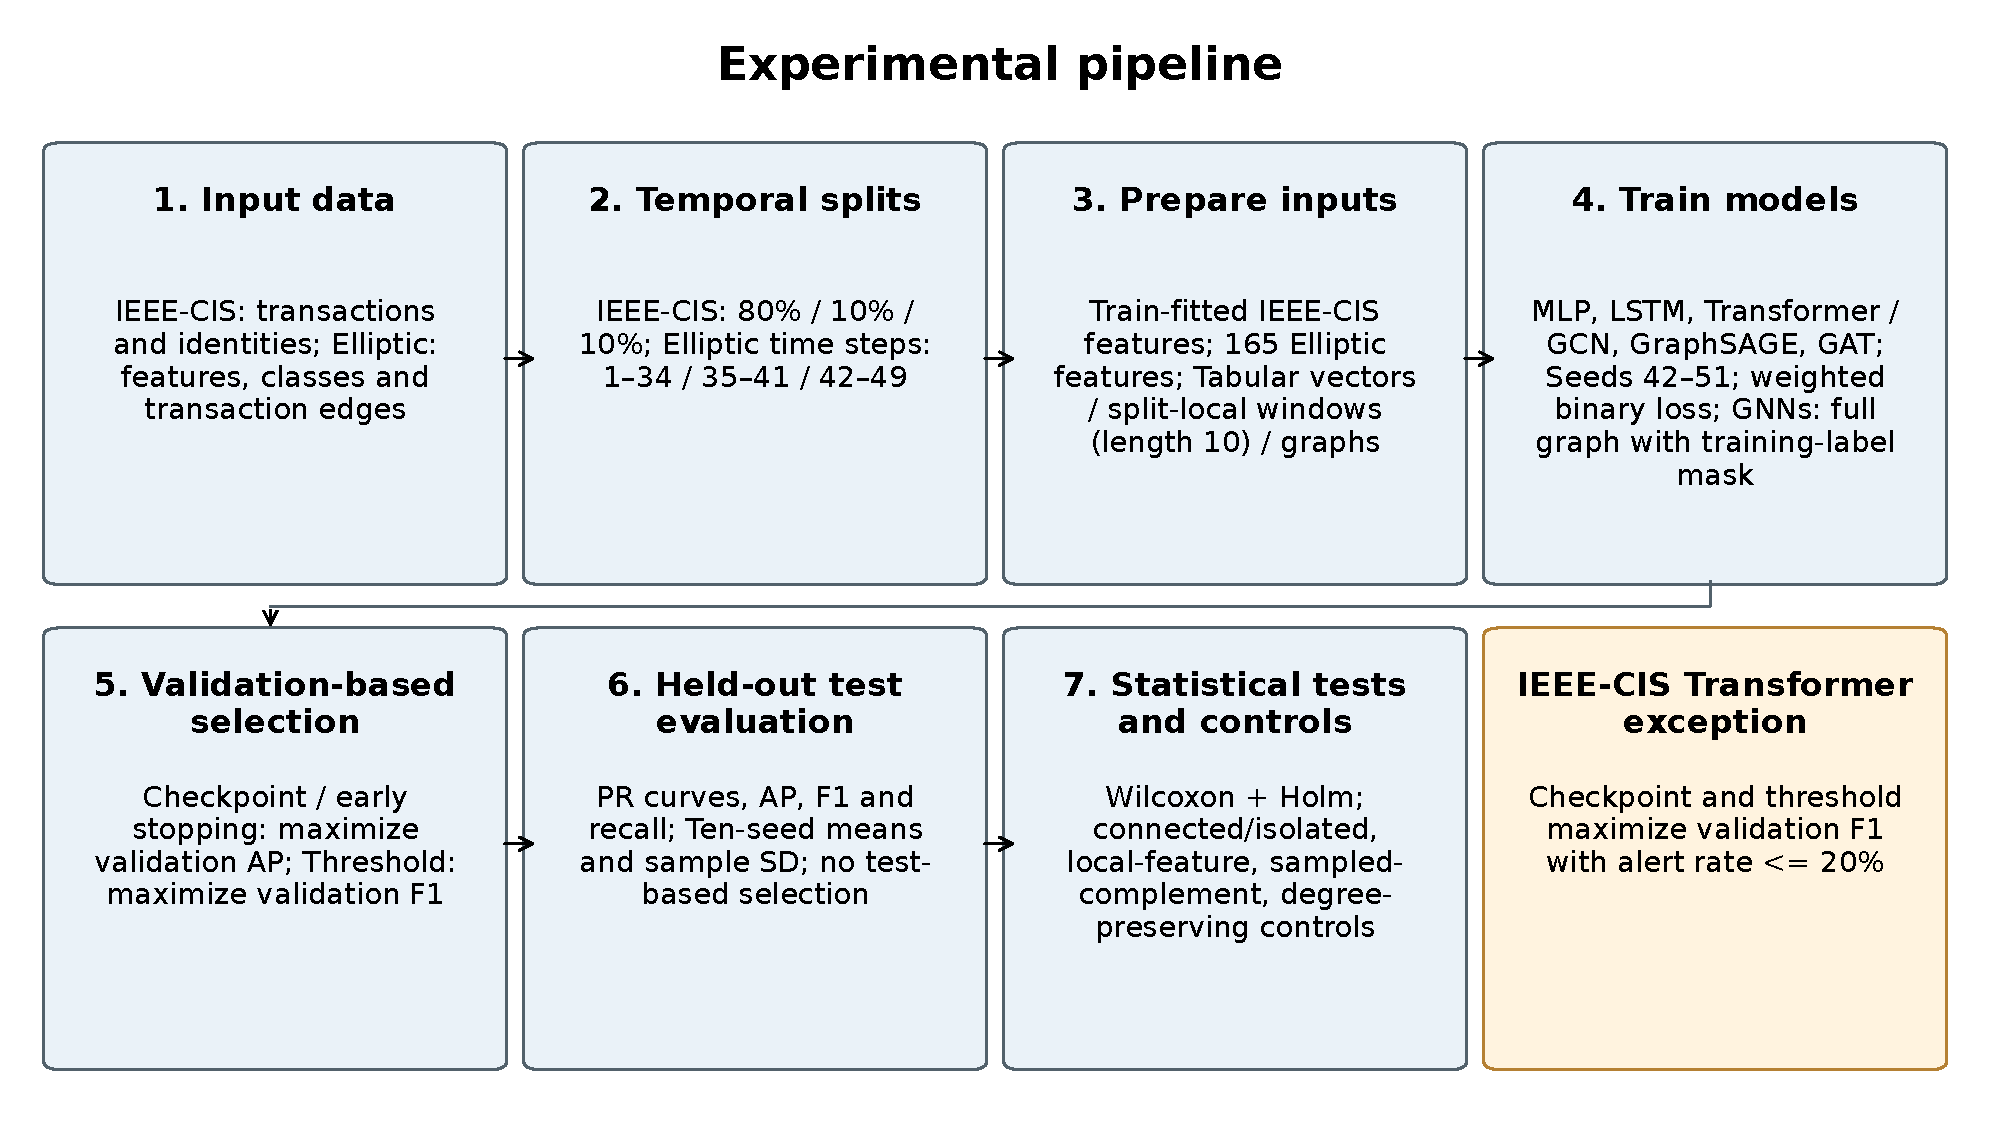
\includegraphics[width=\linewidth]{thesis_figures/slides/01_pipeline.pdf}
\caption{Experimental pipeline. Validation selects checkpoints and thresholds. The IEEE-CIS Transformer instead maximizes validation F1 subject to an alert rate of at most 20\% for both selections. The final stage covers Wilcoxon/Holm tests and the four listed controls.}
\label{fig:01-pipeline}
\end{figure}

\begin{figure}[htbp]
\centering
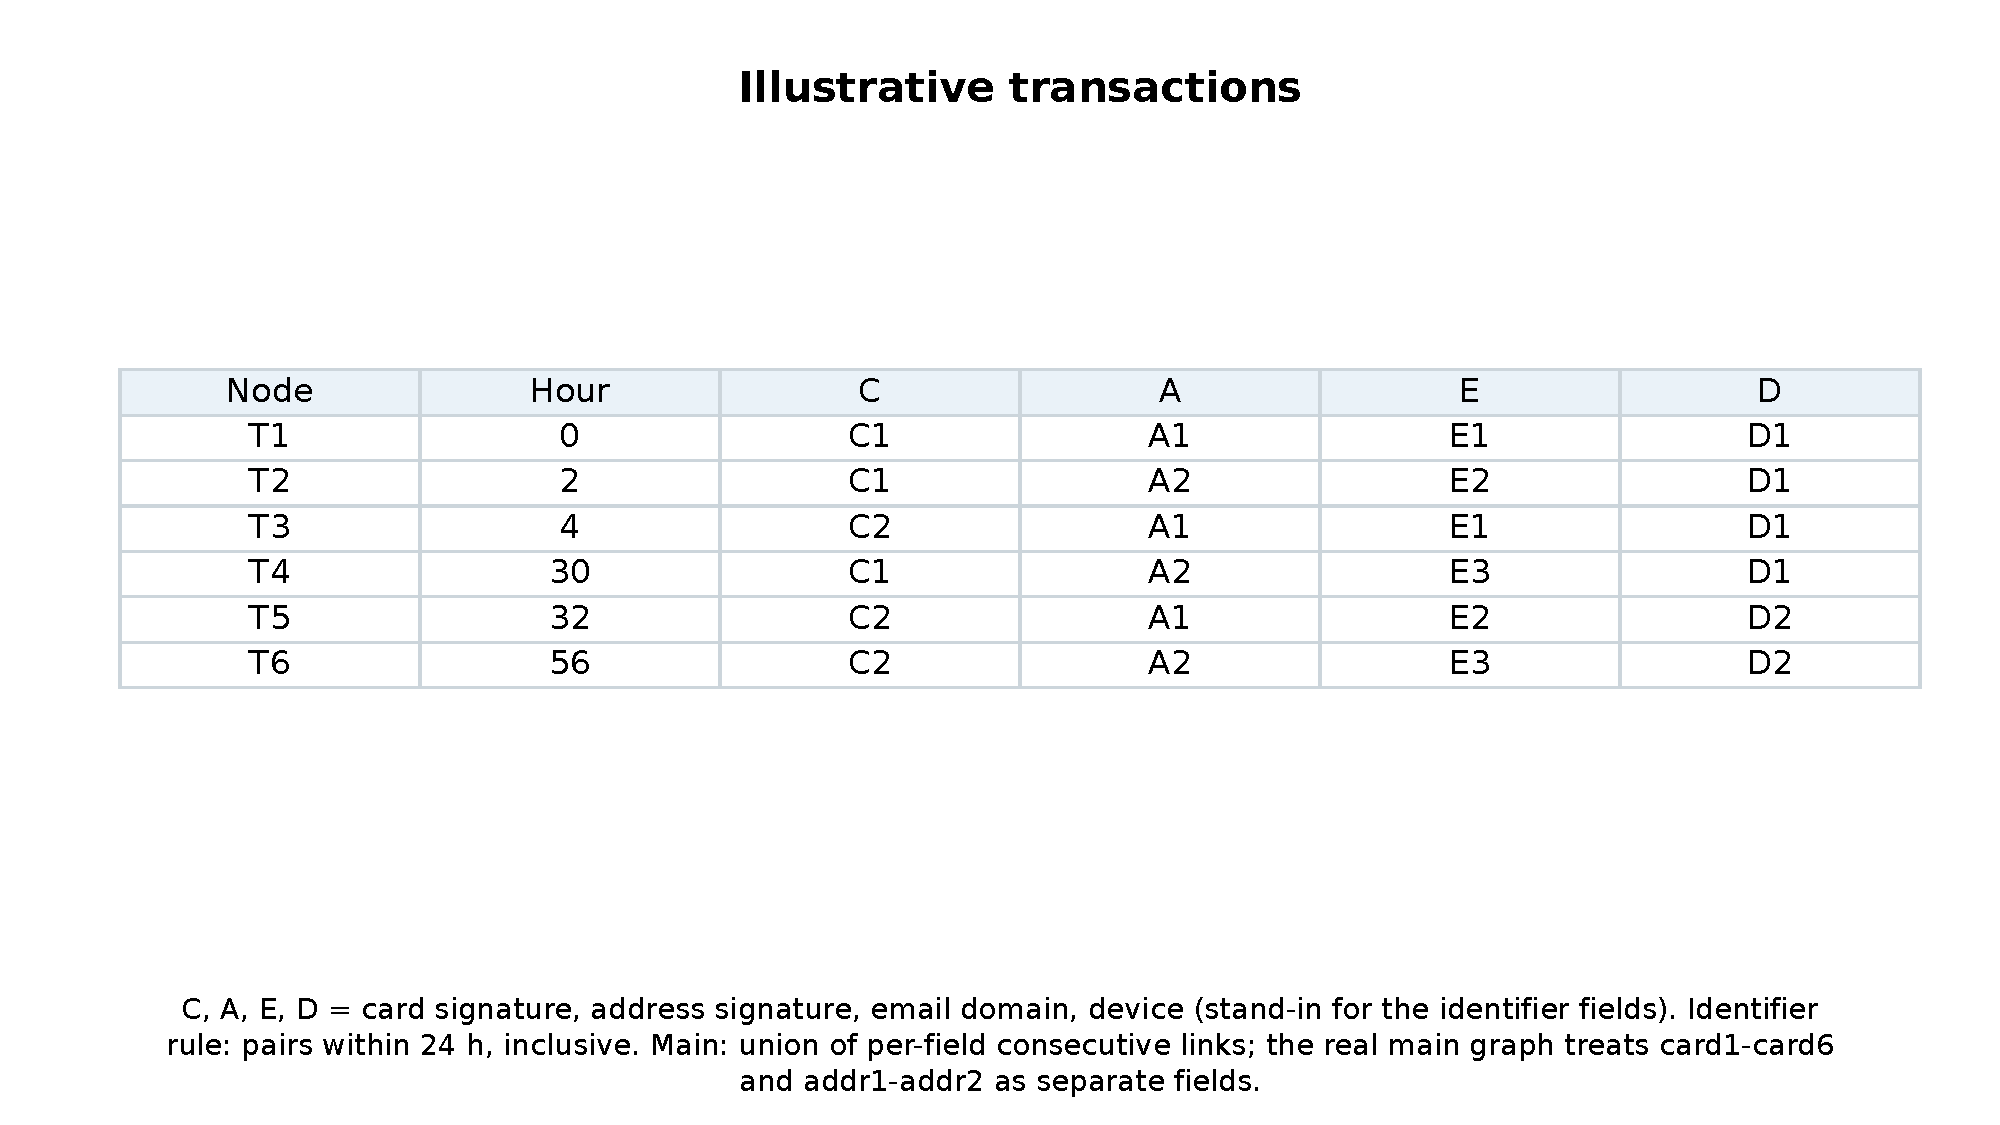
\includegraphics[width=\linewidth]{thesis_figures/slides/transactions/02_graph_constructions.pdf}
\caption{C, A, E, D = card signature, address signature, email domain, device (stand-in for the identifier fields). Identifier rule: pairs within 24 h, inclusive. Main: union of per-field consecutive links; the real main graph treats card1-card6 and addr1-addr2 as separate fields. Synthetic illustration; bidirectional edges are shown once and model self-loops are omitted.}
\label{fig:transactions/02-graph-constructions}
\end{figure}

\begin{figure}[htbp]
\centering
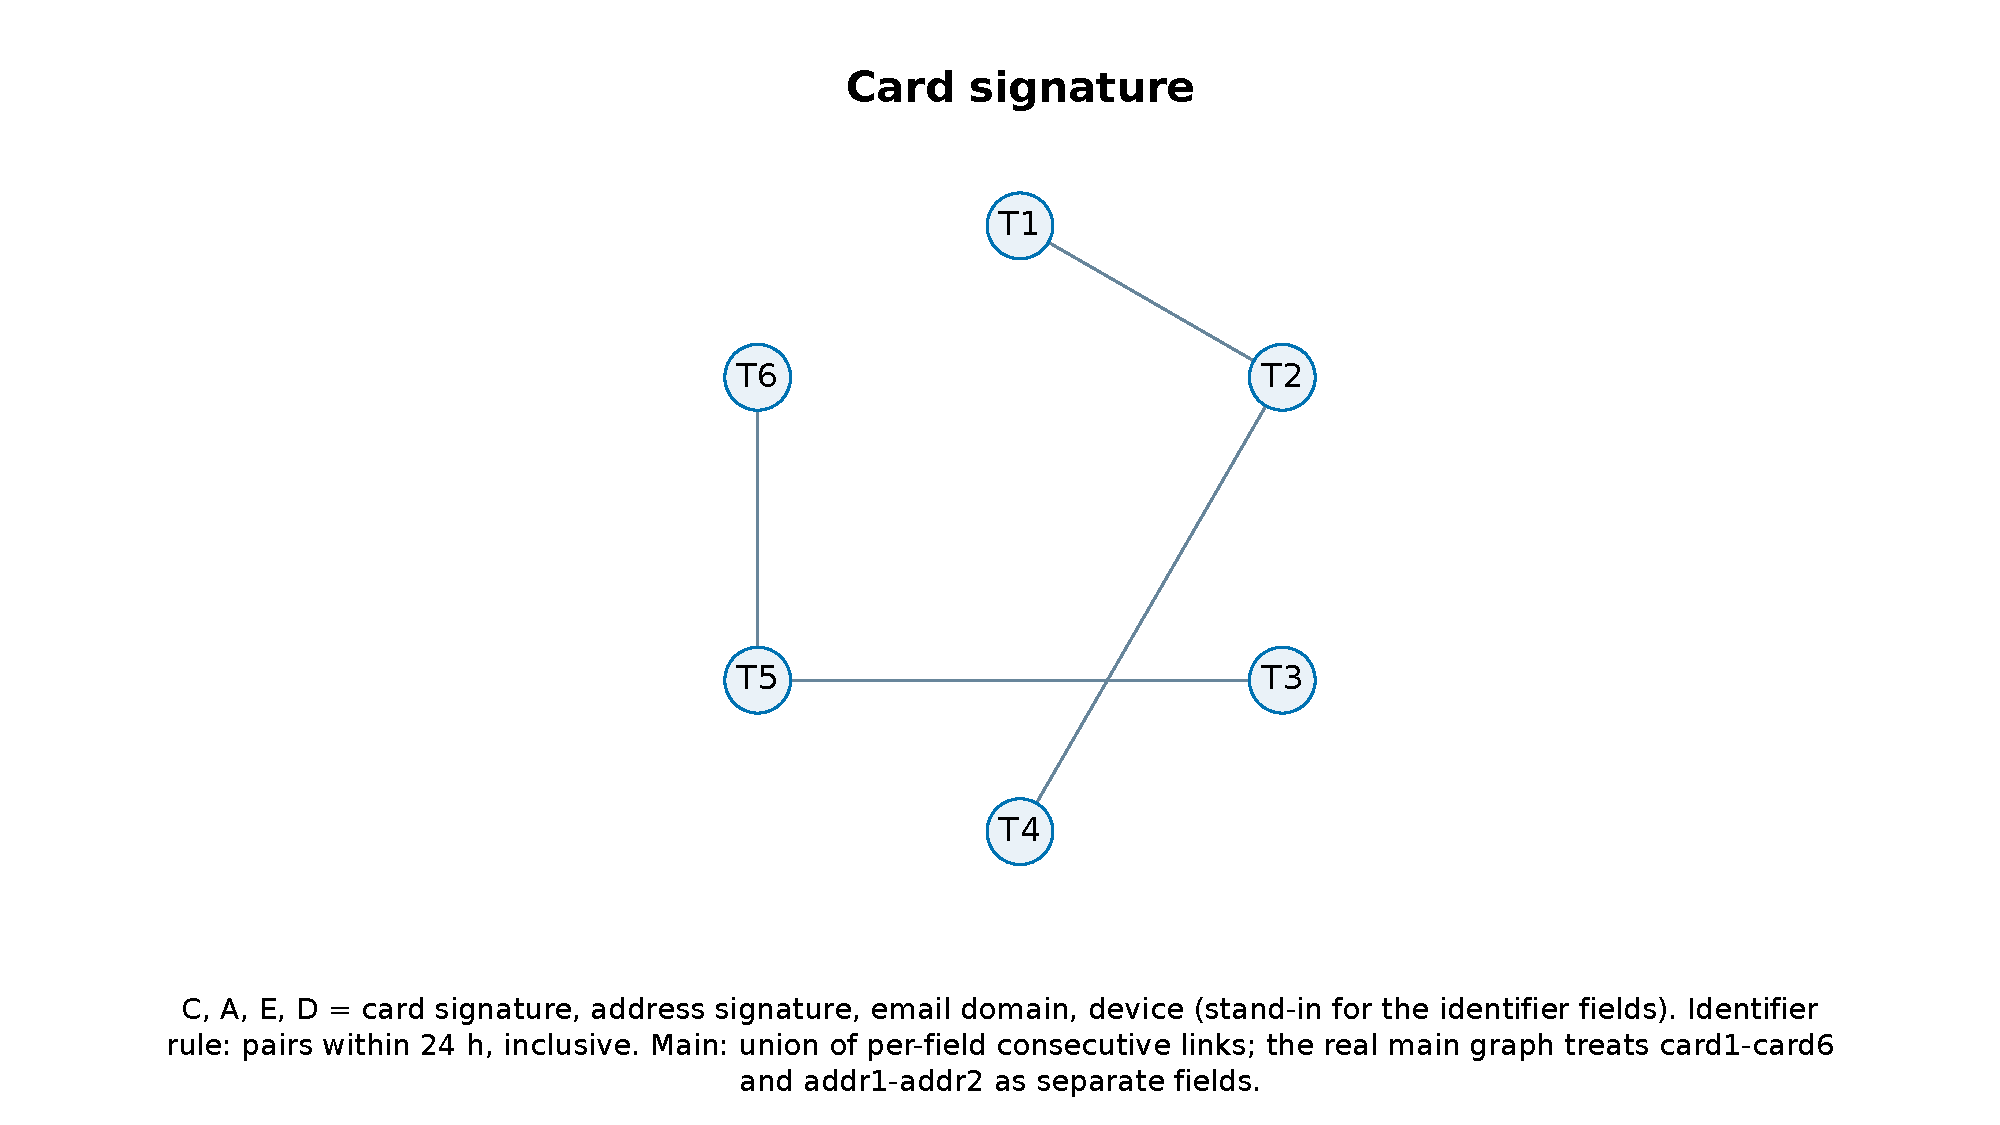
\includegraphics[width=\linewidth]{thesis_figures/slides/card/02_graph_constructions.pdf}
\caption{C, A, E, D = card signature, address signature, email domain, device (stand-in for the identifier fields). Identifier rule: pairs within 24 h, inclusive. Main: union of per-field consecutive links; the real main graph treats card1-card6 and addr1-addr2 as separate fields. Synthetic illustration; bidirectional edges are shown once and model self-loops are omitted.}
\label{fig:card/02-graph-constructions}
\end{figure}

\begin{figure}[htbp]
\centering
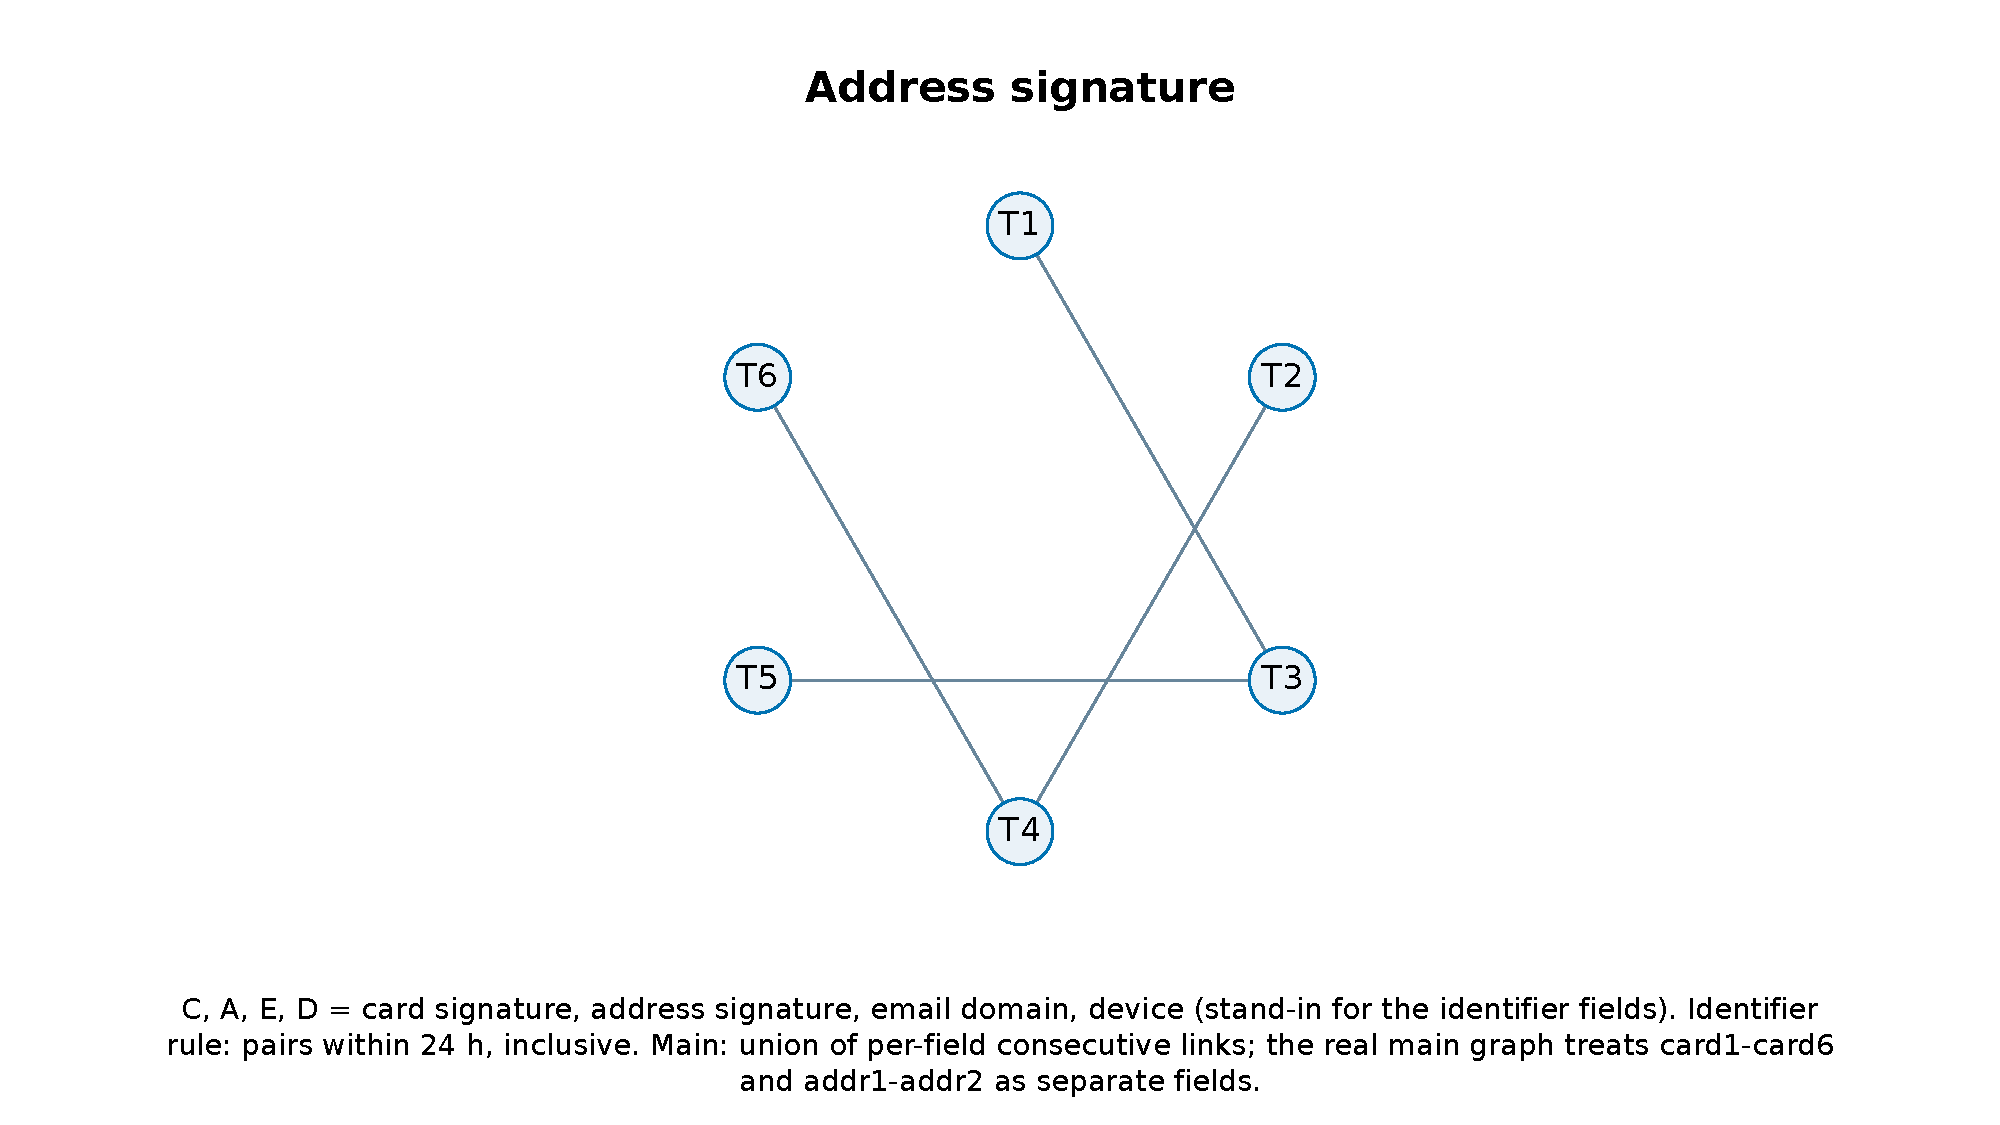
\includegraphics[width=\linewidth]{thesis_figures/slides/address/02_graph_constructions.pdf}
\caption{C, A, E, D = card signature, address signature, email domain, device (stand-in for the identifier fields). Identifier rule: pairs within 24 h, inclusive. Main: union of per-field consecutive links; the real main graph treats card1-card6 and addr1-addr2 as separate fields. Synthetic illustration; bidirectional edges are shown once and model self-loops are omitted.}
\label{fig:address/02-graph-constructions}
\end{figure}

\begin{figure}[htbp]
\centering
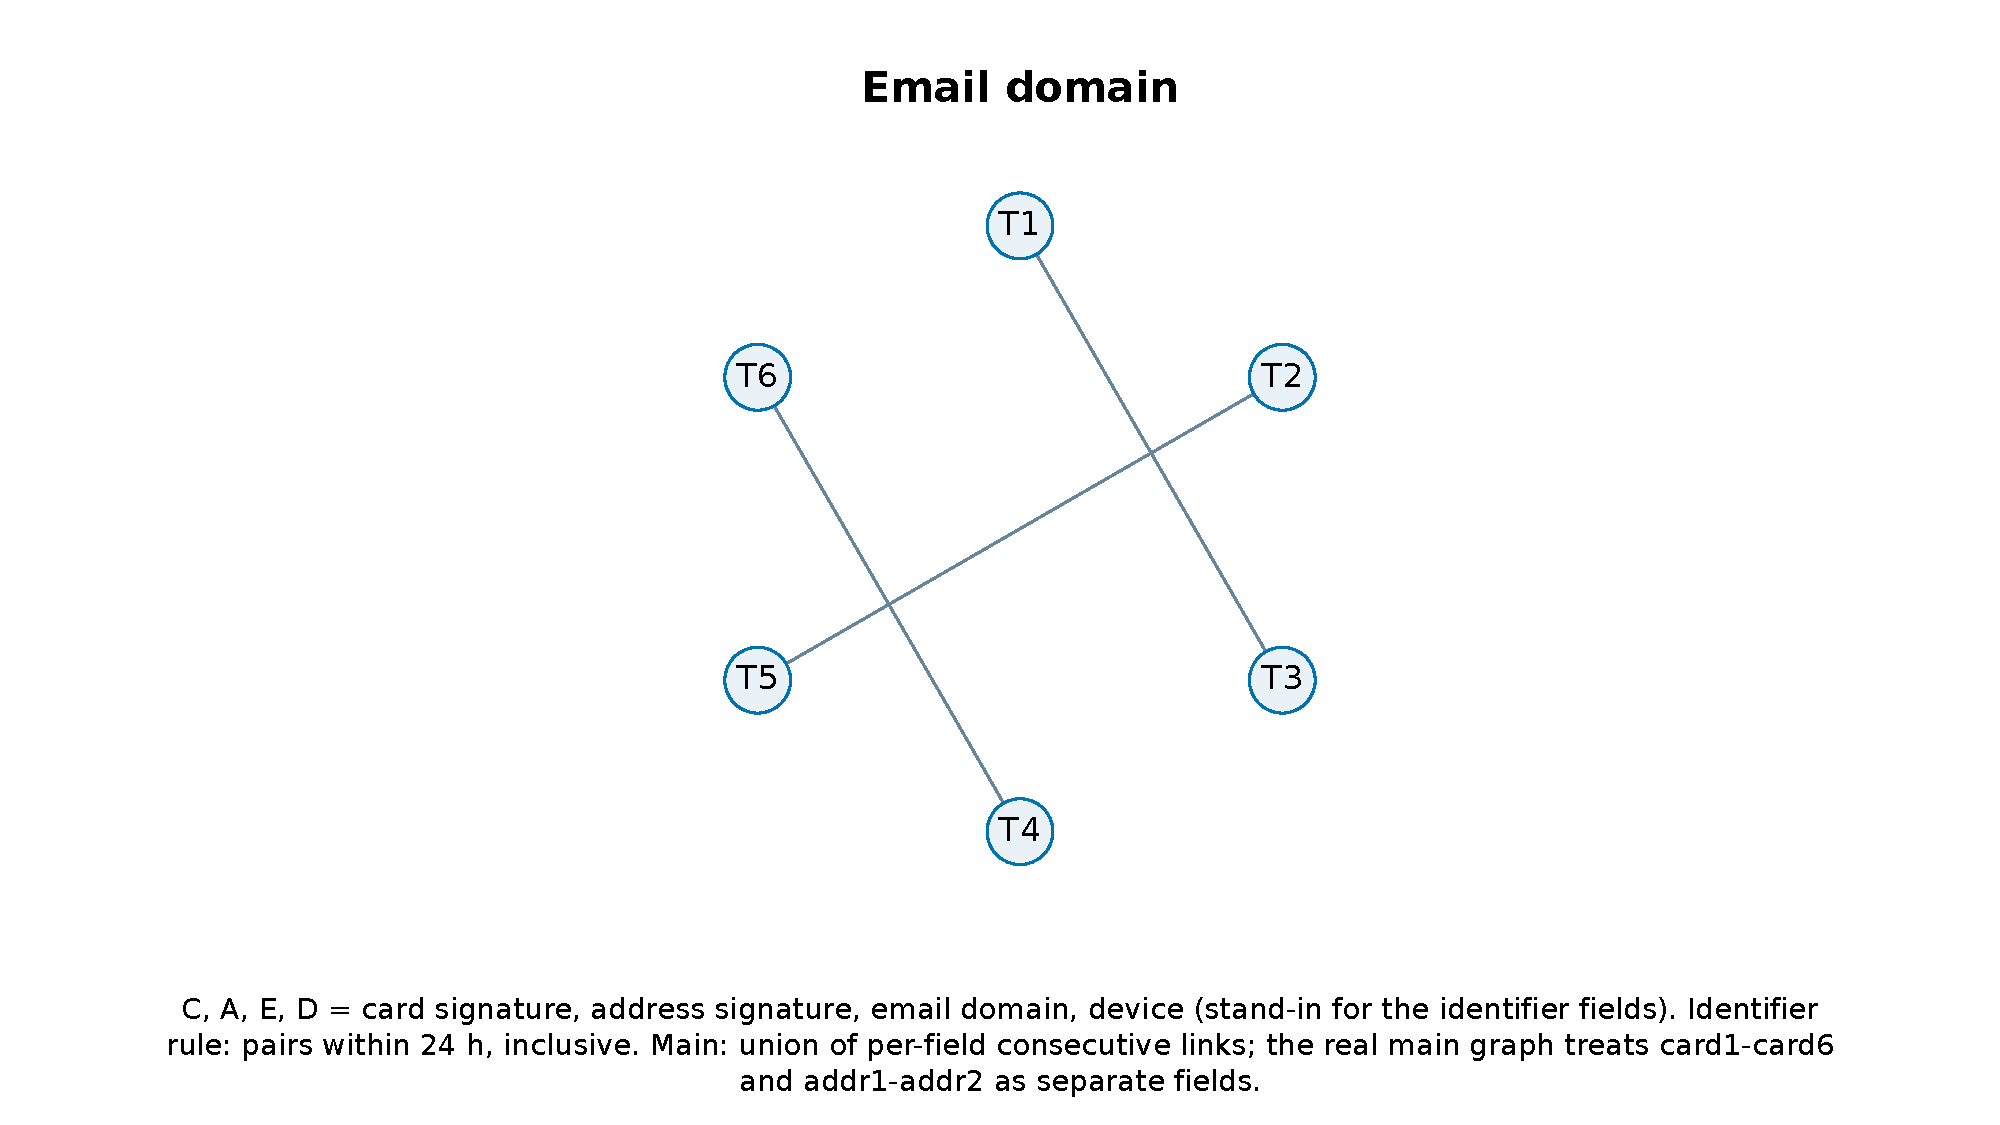
\includegraphics[width=\linewidth]{thesis_figures/slides/email/02_graph_constructions.pdf}
\caption{C, A, E, D = card signature, address signature, email domain, device (stand-in for the identifier fields). Identifier rule: pairs within 24 h, inclusive. Main: union of per-field consecutive links; the real main graph treats card1-card6 and addr1-addr2 as separate fields. Synthetic illustration; bidirectional edges are shown once and model self-loops are omitted.}
\label{fig:email/02-graph-constructions}
\end{figure}

\begin{figure}[htbp]
\centering
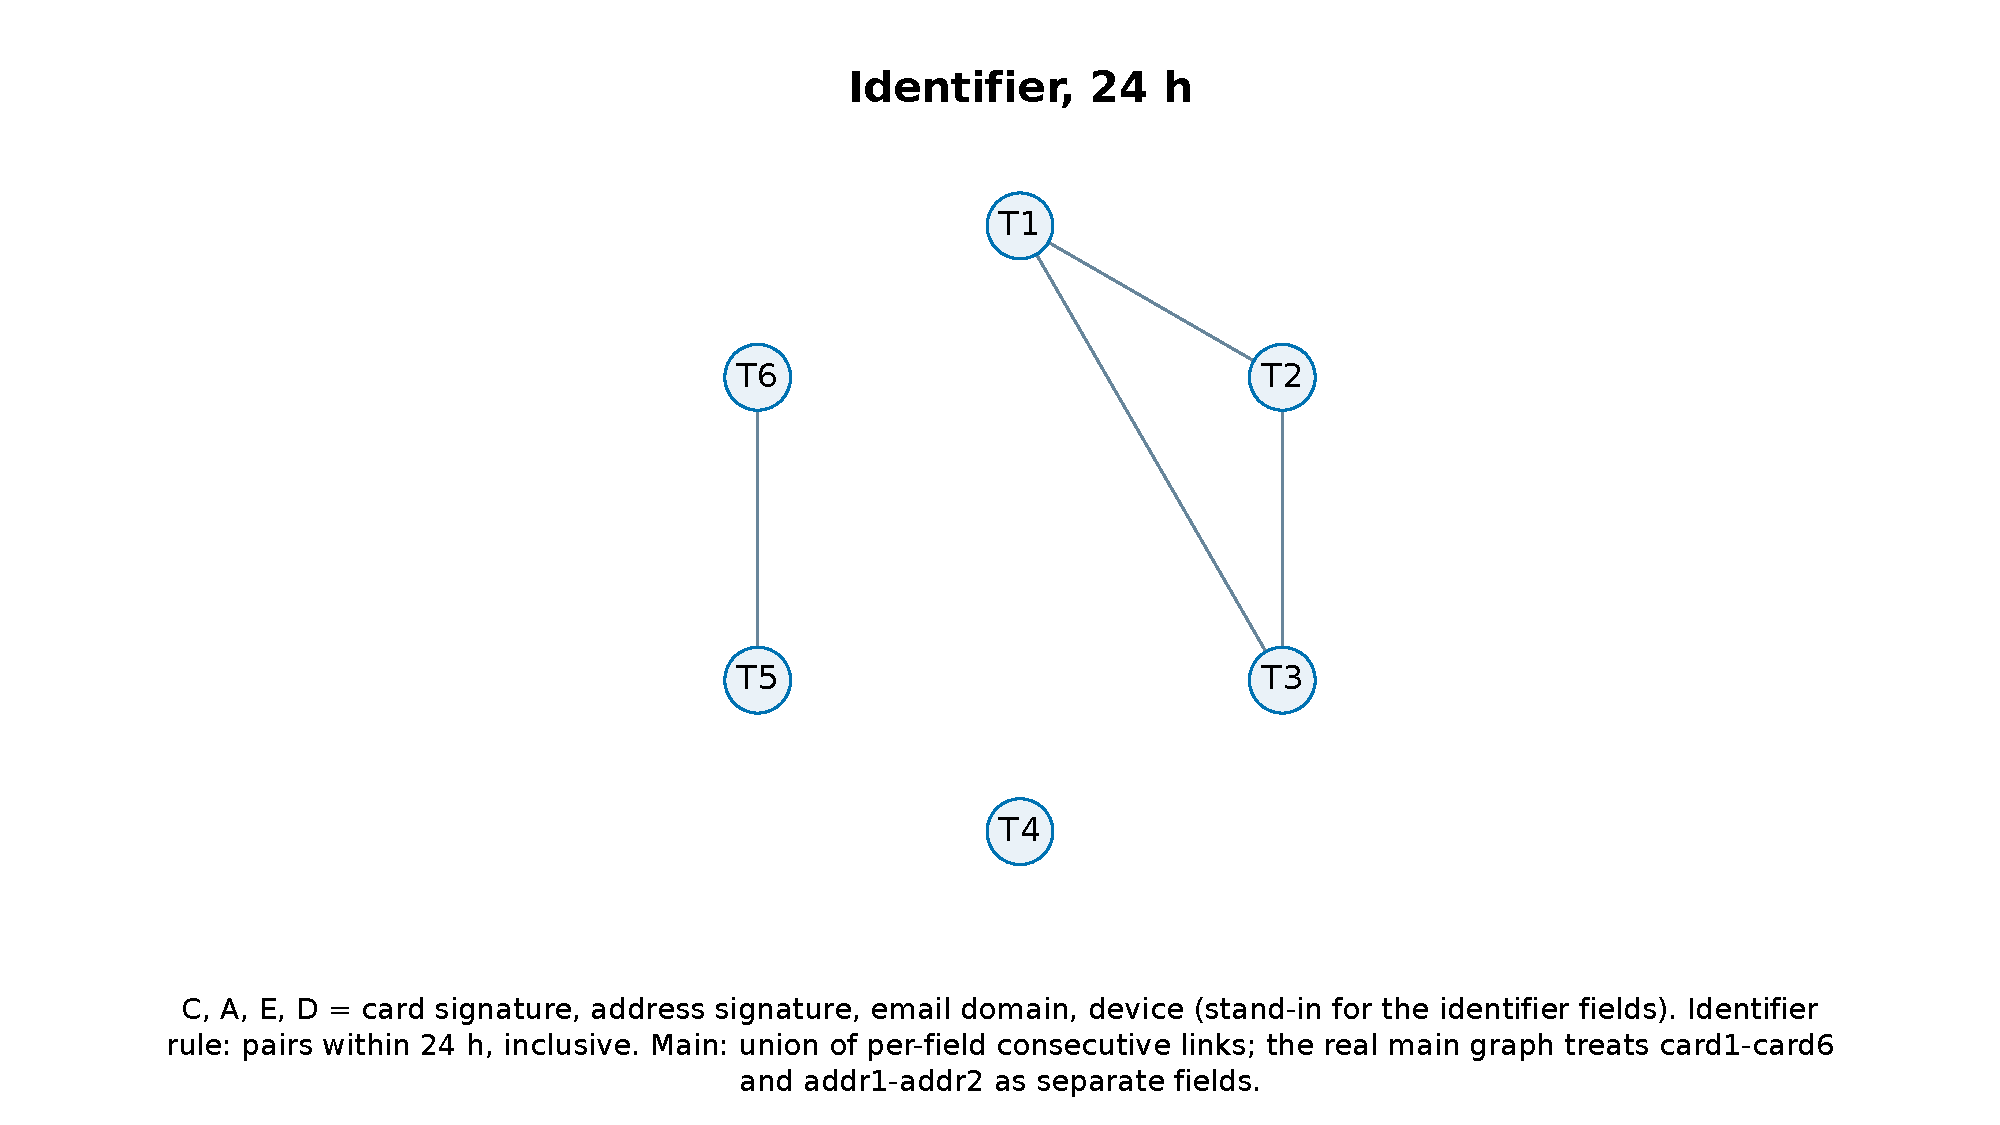
\includegraphics[width=\linewidth]{thesis_figures/slides/identifier/02_graph_constructions.pdf}
\caption{C, A, E, D = card signature, address signature, email domain, device (stand-in for the identifier fields). Identifier rule: pairs within 24 h, inclusive. Main: union of per-field consecutive links; the real main graph treats card1-card6 and addr1-addr2 as separate fields. Synthetic illustration; bidirectional edges are shown once and model self-loops are omitted.}
\label{fig:identifier/02-graph-constructions}
\end{figure}

\begin{figure}[htbp]
\centering
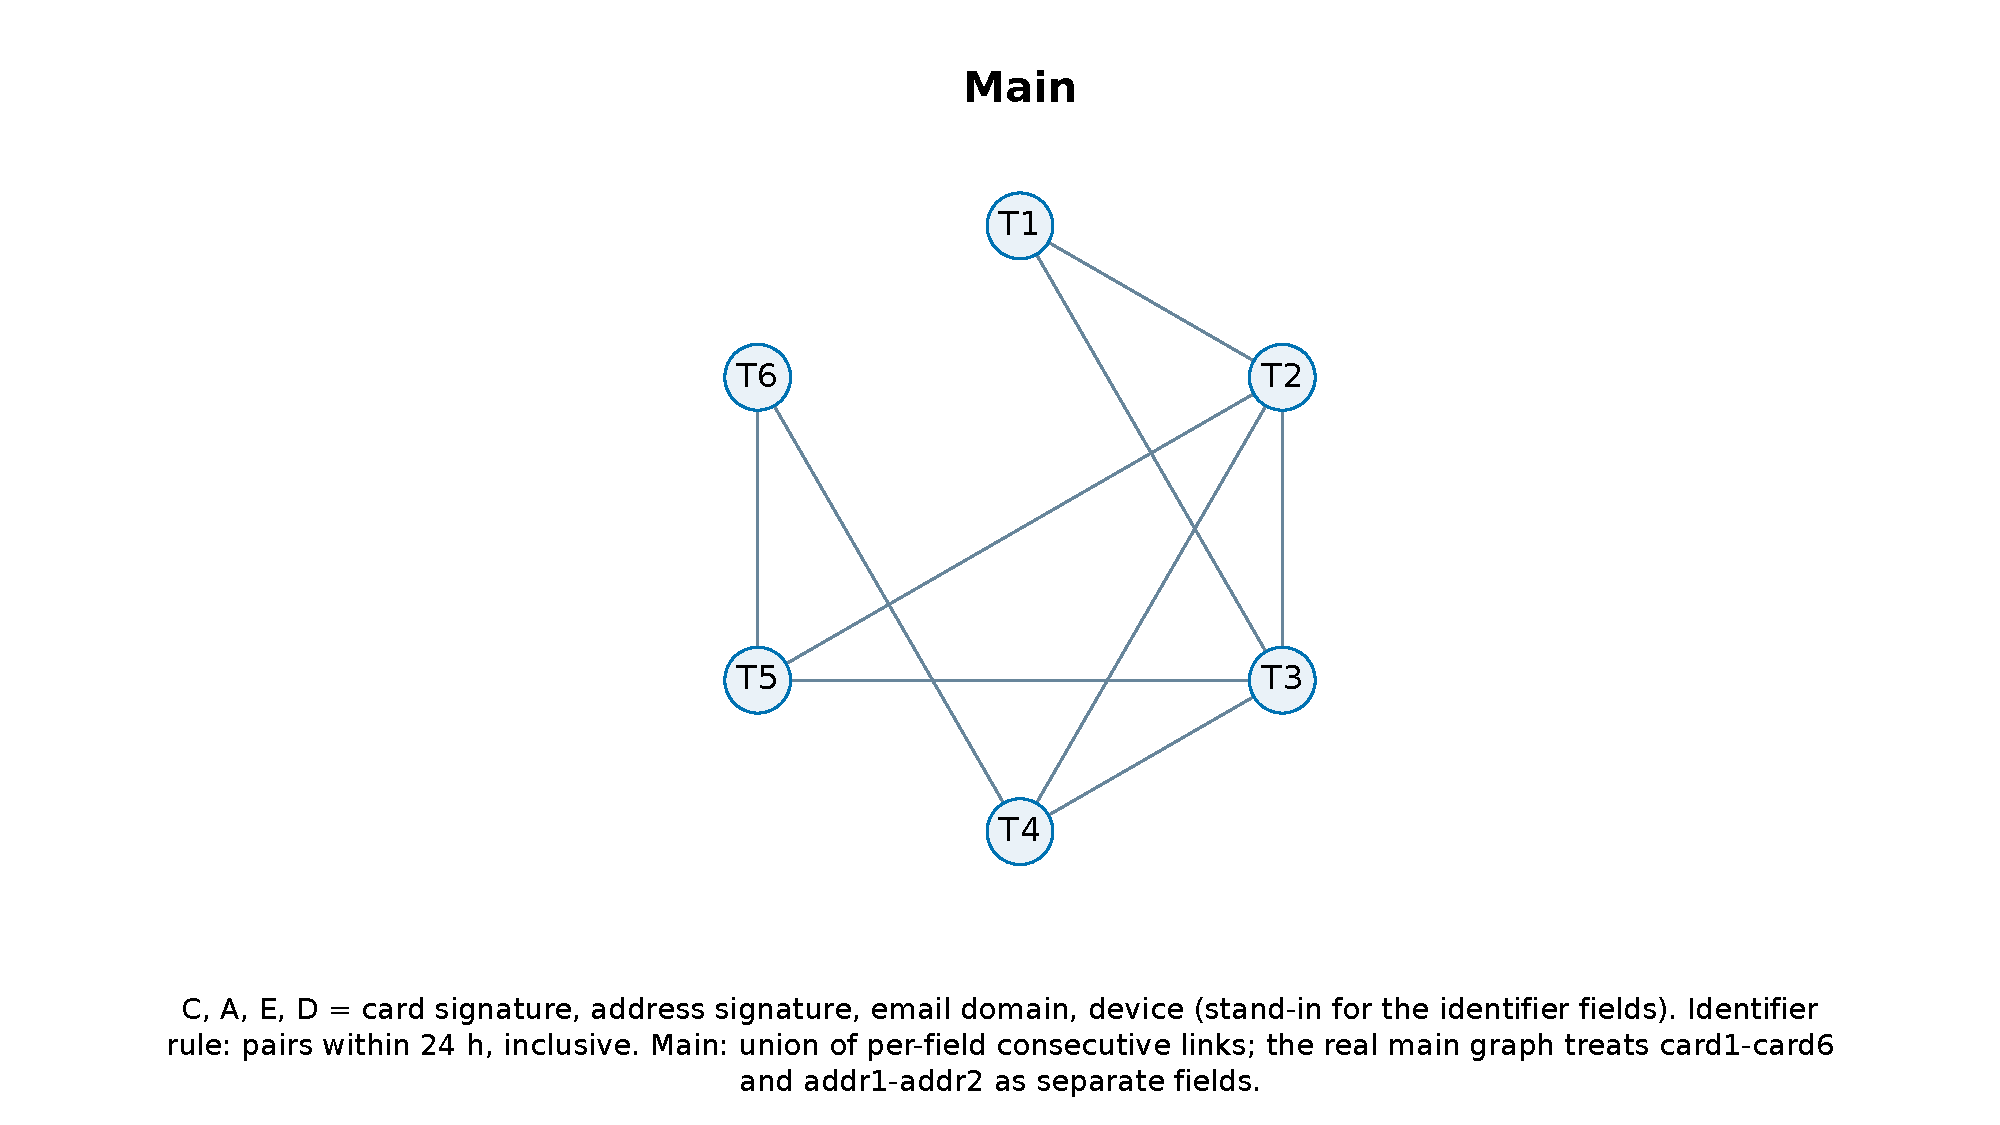
\includegraphics[width=\linewidth]{thesis_figures/slides/main/02_graph_constructions.pdf}
\caption{C, A, E, D = card signature, address signature, email domain, device (stand-in for the identifier fields). Identifier rule: pairs within 24 h, inclusive. Main: union of per-field consecutive links; the real main graph treats card1-card6 and addr1-addr2 as separate fields. Synthetic illustration; bidirectional edges are shown once and model self-loops are omitted.}
\label{fig:main/02-graph-constructions}
\end{figure}

\begin{figure}[htbp]
\centering
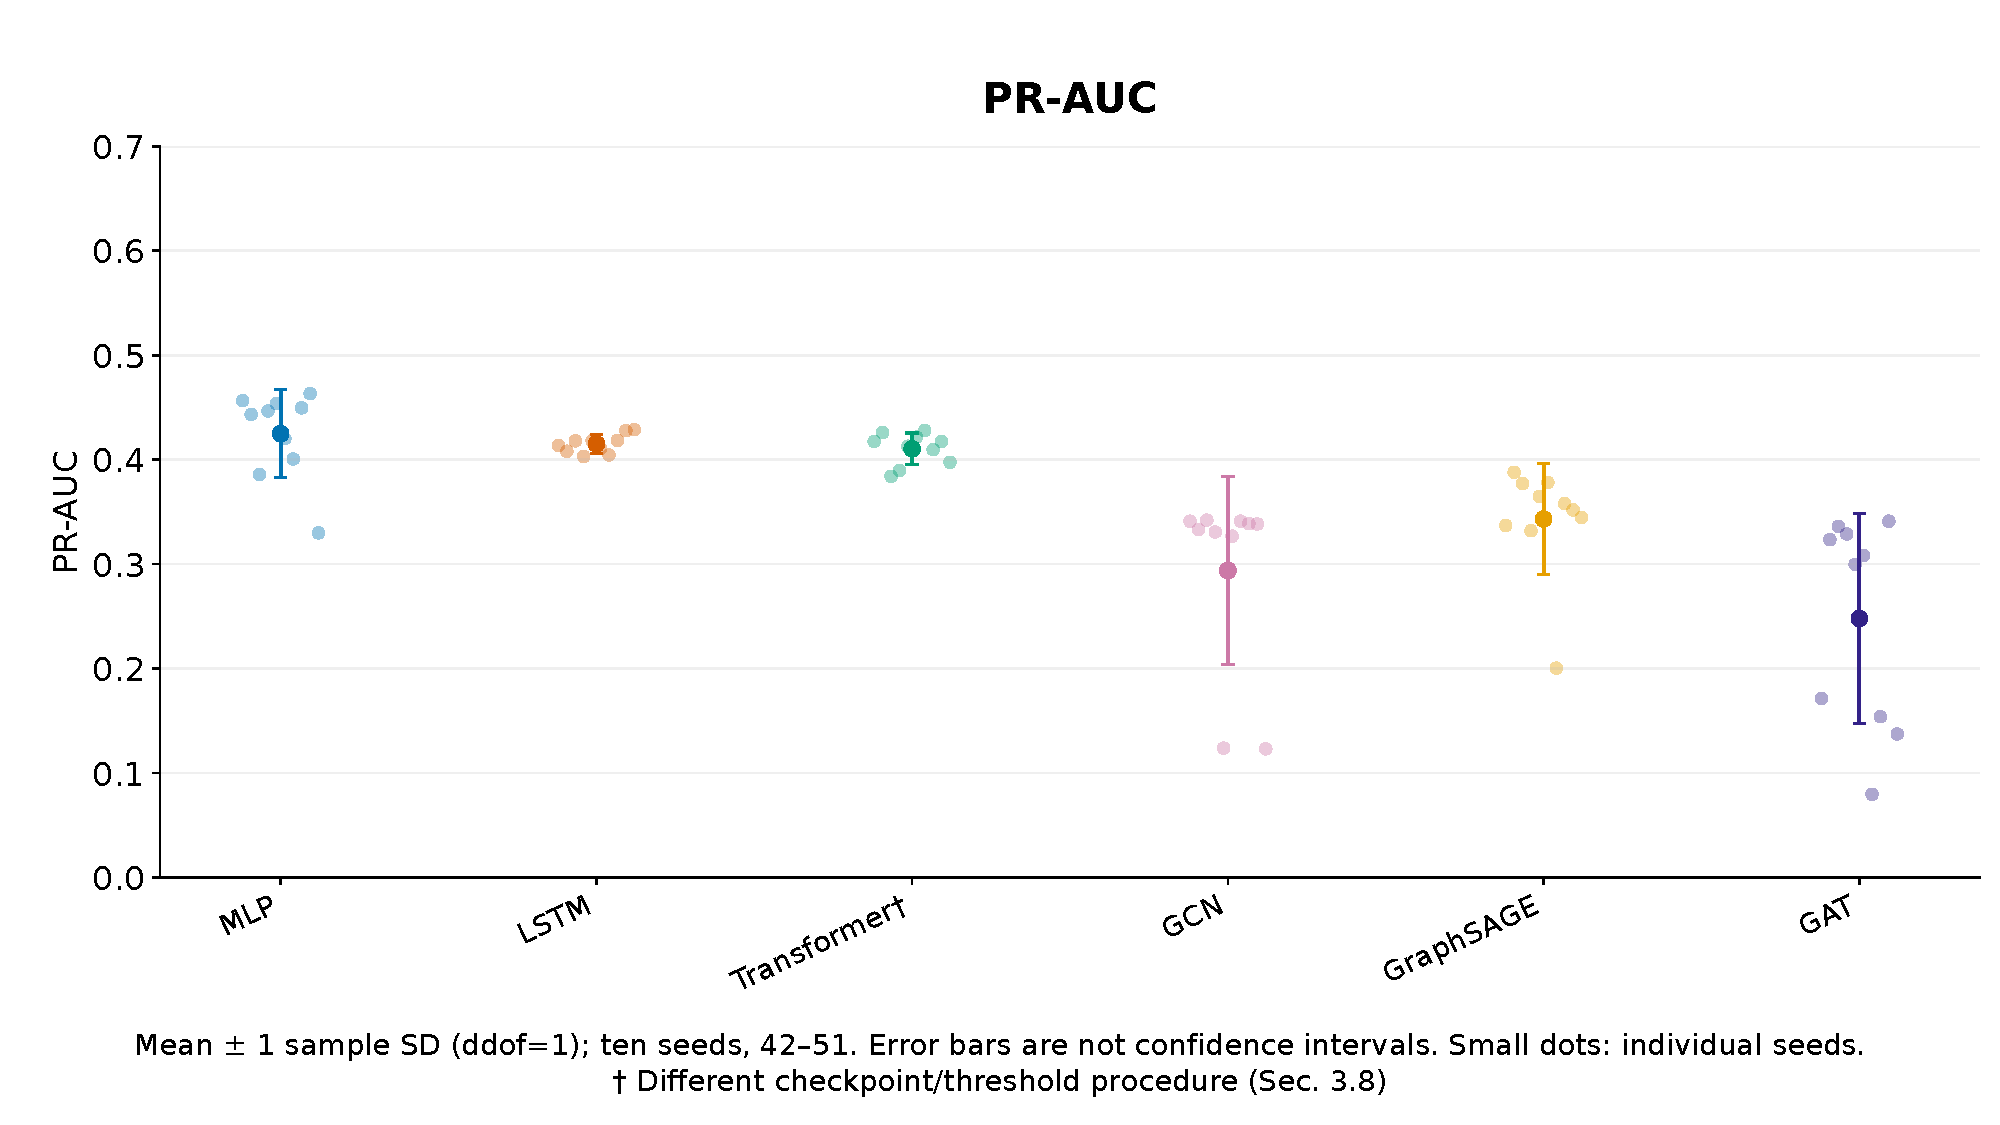
\includegraphics[width=\linewidth]{thesis_figures/slides/pr_auc/03_results_ieee-cis.pdf}
\caption{IEEE-CIS: ten-seed means $\pm$ sample SD; GNNs use the main graph. AP is average precision. F1 and recall use validation-selected thresholds. † Different checkpoint/threshold procedure (Sec. 3.8).}
\label{fig:pr-auc/03-results-ieee-cis}
\end{figure}

\begin{figure}[htbp]
\centering
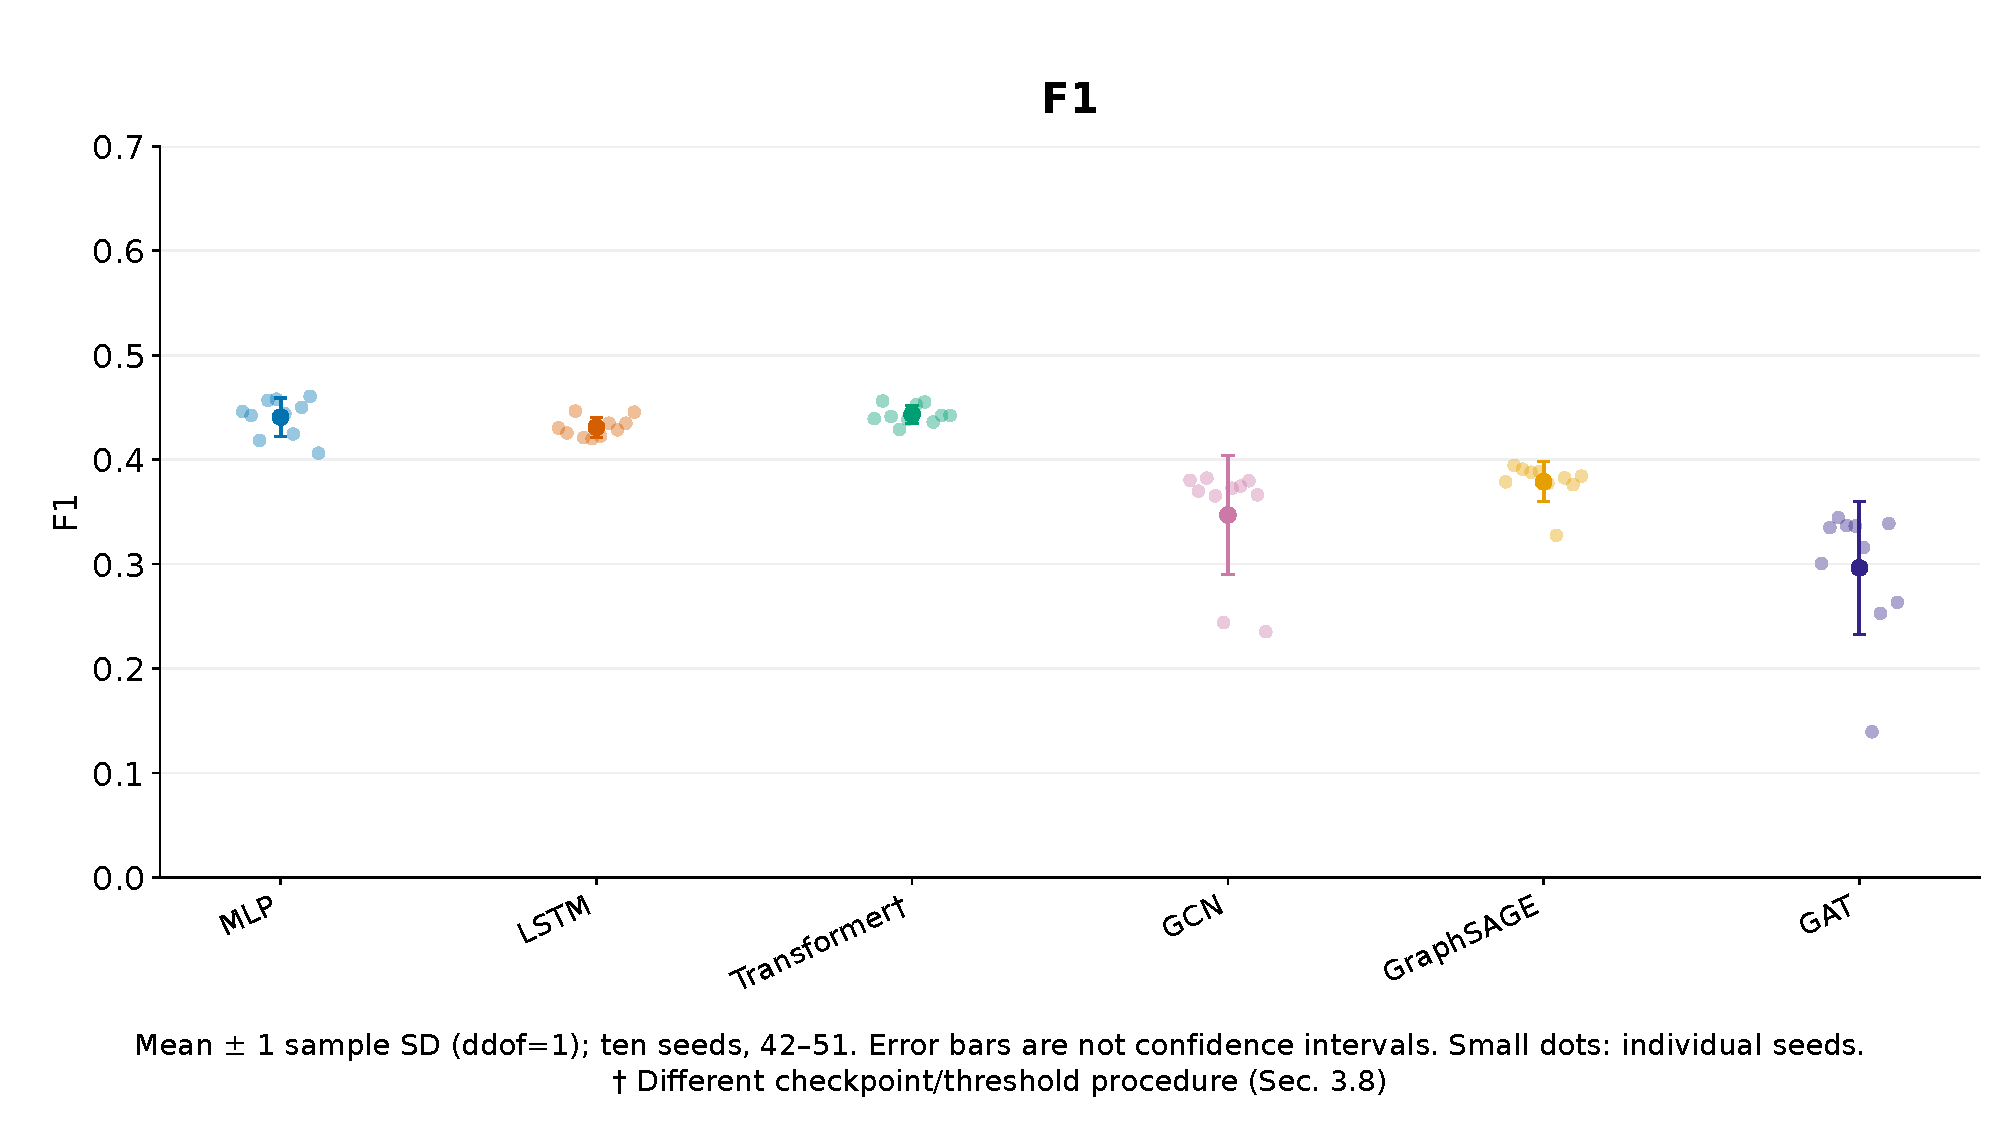
\includegraphics[width=\linewidth]{thesis_figures/slides/f1_score/03_results_ieee-cis.pdf}
\caption{IEEE-CIS: ten-seed means $\pm$ sample SD; GNNs use the main graph. AP is average precision. F1 and recall use validation-selected thresholds. † Different checkpoint/threshold procedure (Sec. 3.8).}
\label{fig:f1-score/03-results-ieee-cis}
\end{figure}

\begin{figure}[htbp]
\centering
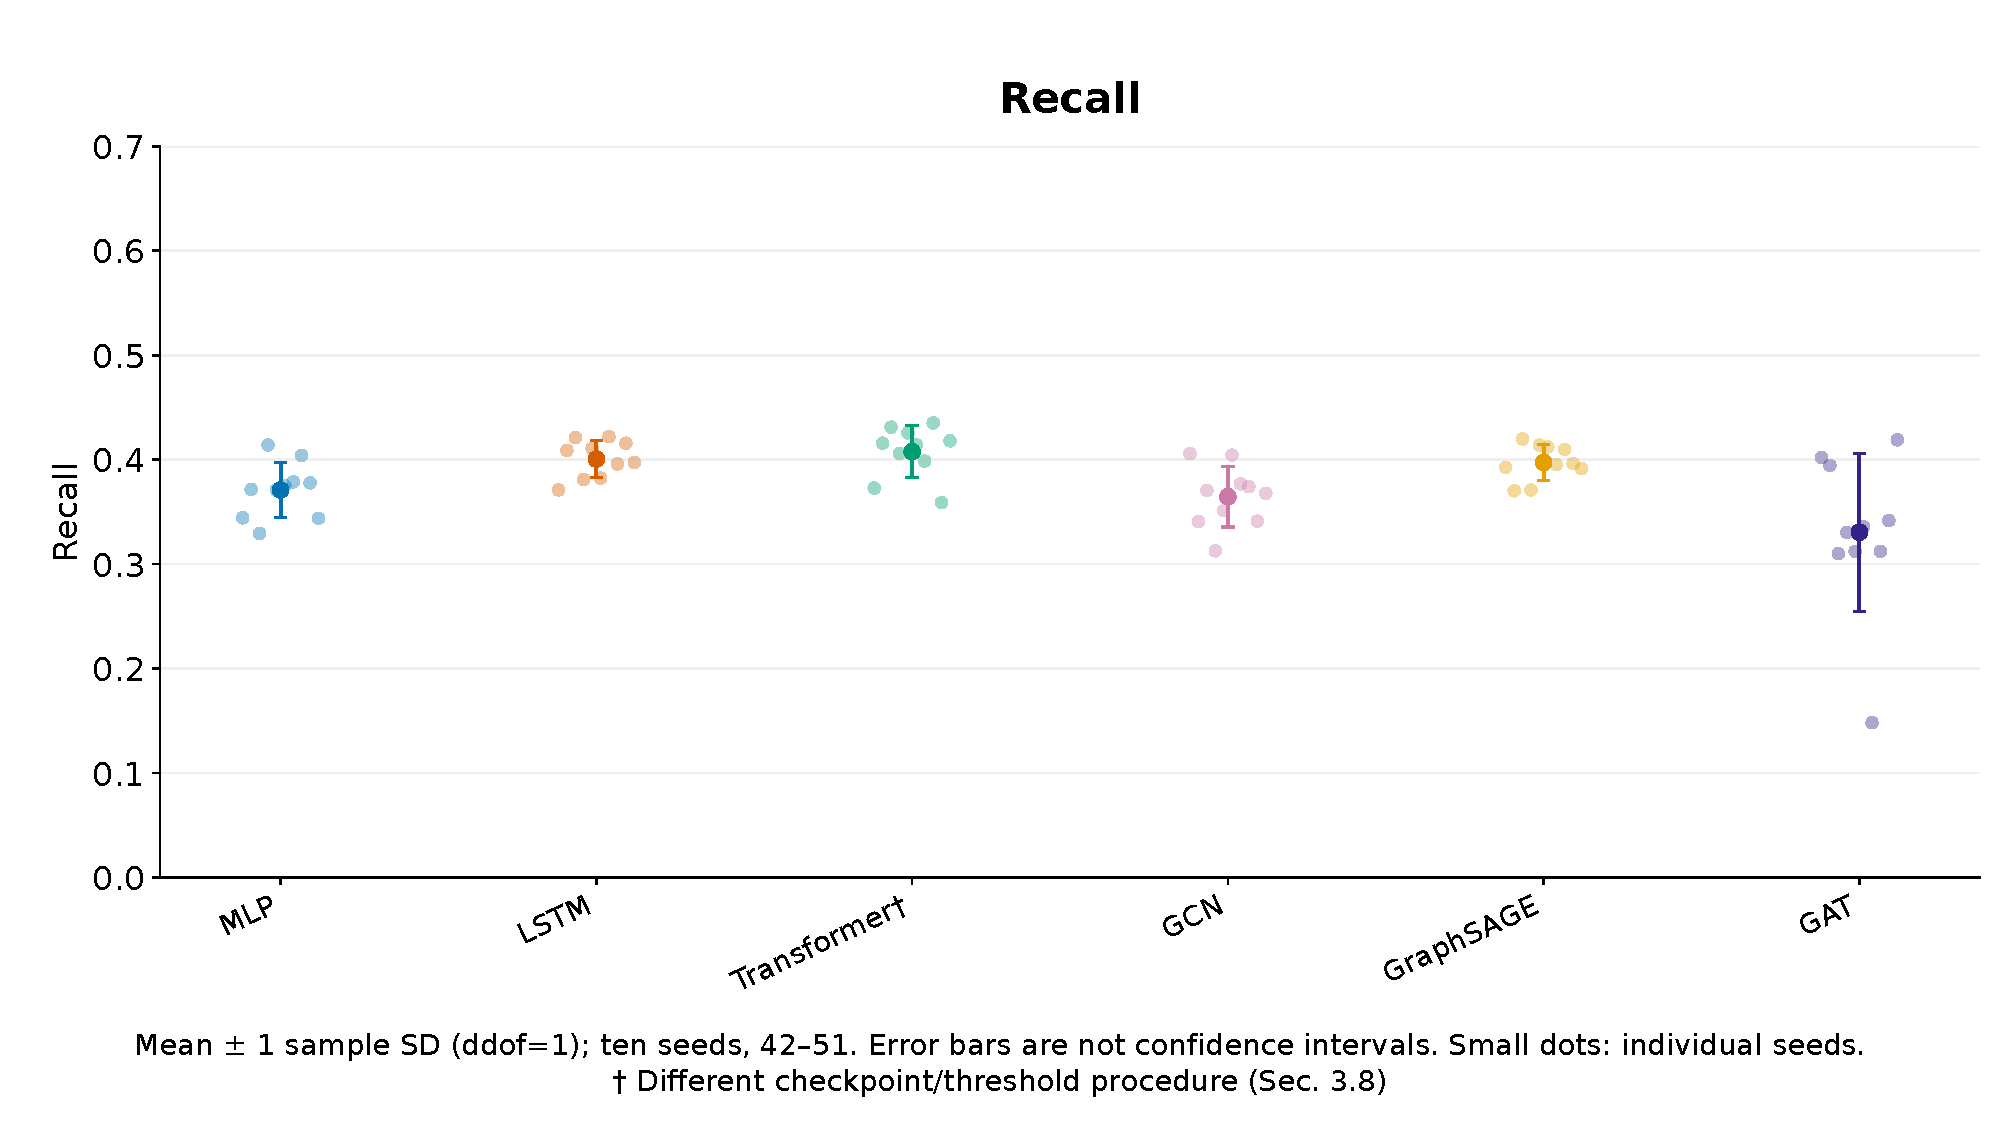
\includegraphics[width=\linewidth]{thesis_figures/slides/recall/03_results_ieee-cis.pdf}
\caption{IEEE-CIS: ten-seed means $\pm$ sample SD; GNNs use the main graph. AP is average precision. F1 and recall use validation-selected thresholds. † Different checkpoint/threshold procedure (Sec. 3.8).}
\label{fig:recall/03-results-ieee-cis}
\end{figure}

\begin{figure}[htbp]
\centering
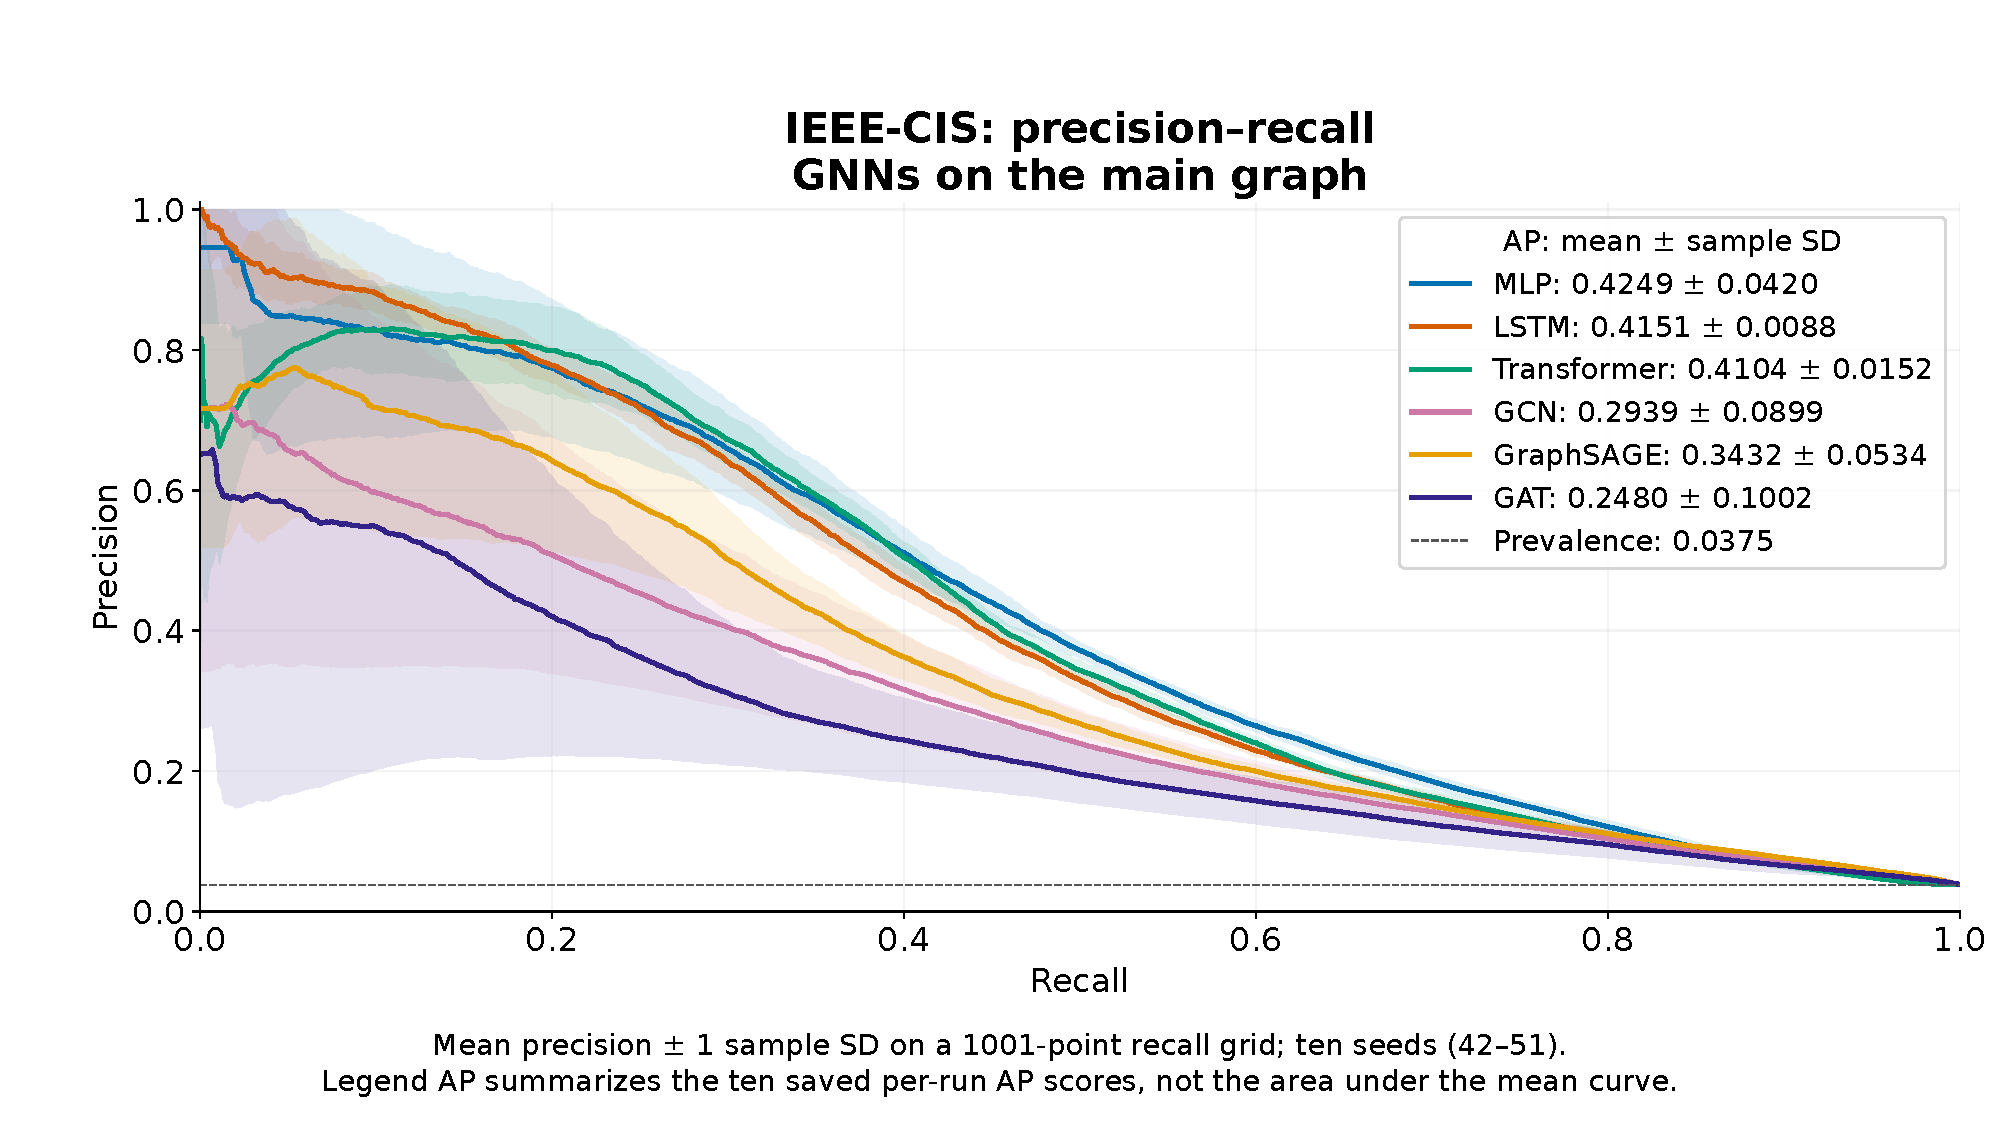
\includegraphics[width=\linewidth]{thesis_figures/slides/04_pr_curves_ieee-cis.pdf}
\caption{IEEE-CIS; GNNs on the main graph. Mean precision curve and $\pm$1 sample-SD band across seeds 42--51, interpolated on 1001 common recall points. The synthetic (recall=0, precision=1) endpoint is removed first; at duplicate recall levels the first reversed point is retained, with constant endpoint extrapolation. Bands are clipped to [0,1]. Legend AP is the mean $\pm$ sample SD of the saved per-run AP scores, matching the ten-seed result tables; it is not the integrated mean curve. Each curve uses its validation-selected checkpoint; checkpoint paths and hashes appear in pr\_curve\_sources.csv.}
\label{fig:04-pr-curves-ieee-cis}
\end{figure}

\begin{figure}[htbp]
\centering
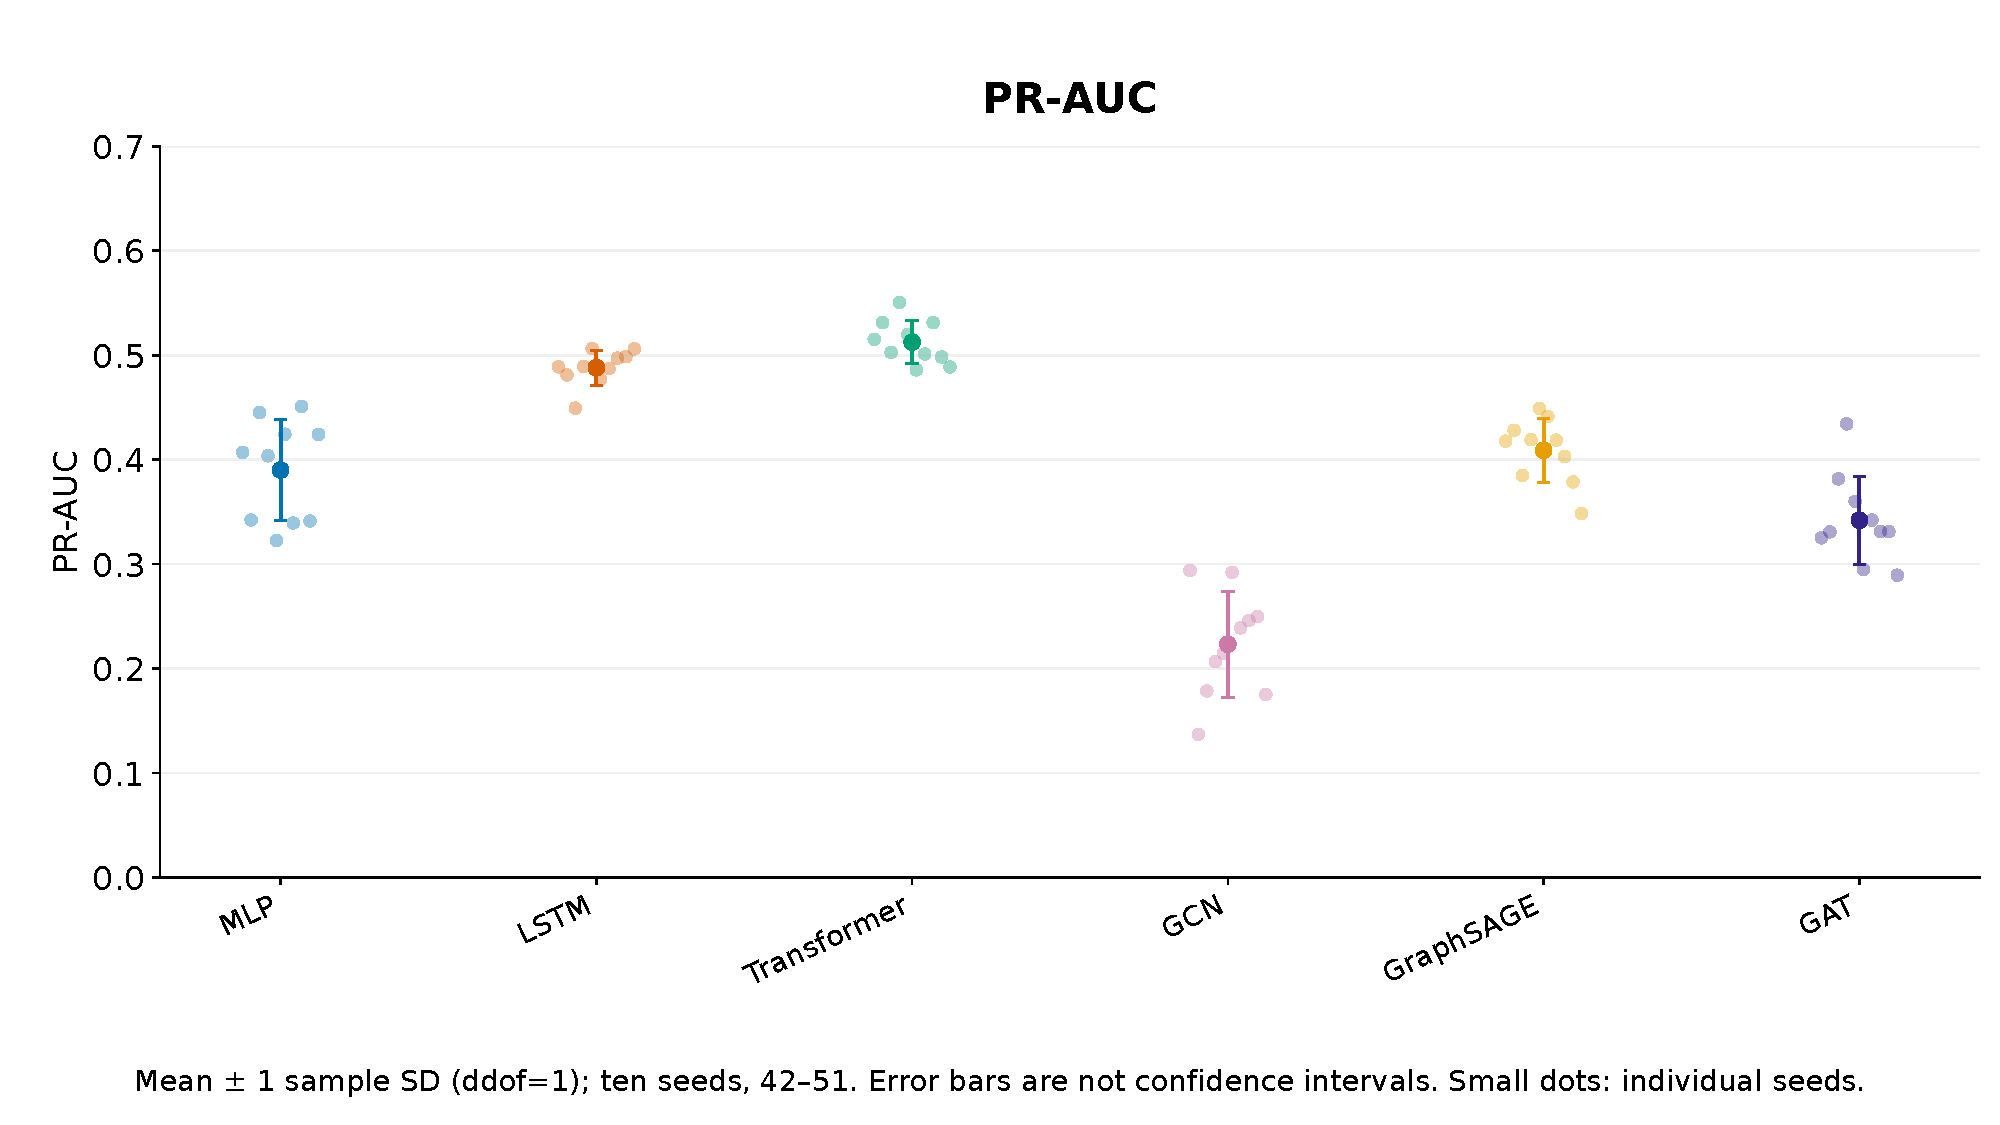
\includegraphics[width=\linewidth]{thesis_figures/slides/pr_auc/03_results_elliptic.pdf}
\caption{Elliptic: ten-seed means $\pm$ sample SD; GNNs use the native graph. AP is average precision. F1 and recall use validation-selected thresholds. }
\label{fig:pr-auc/03-results-elliptic}
\end{figure}

\begin{figure}[htbp]
\centering
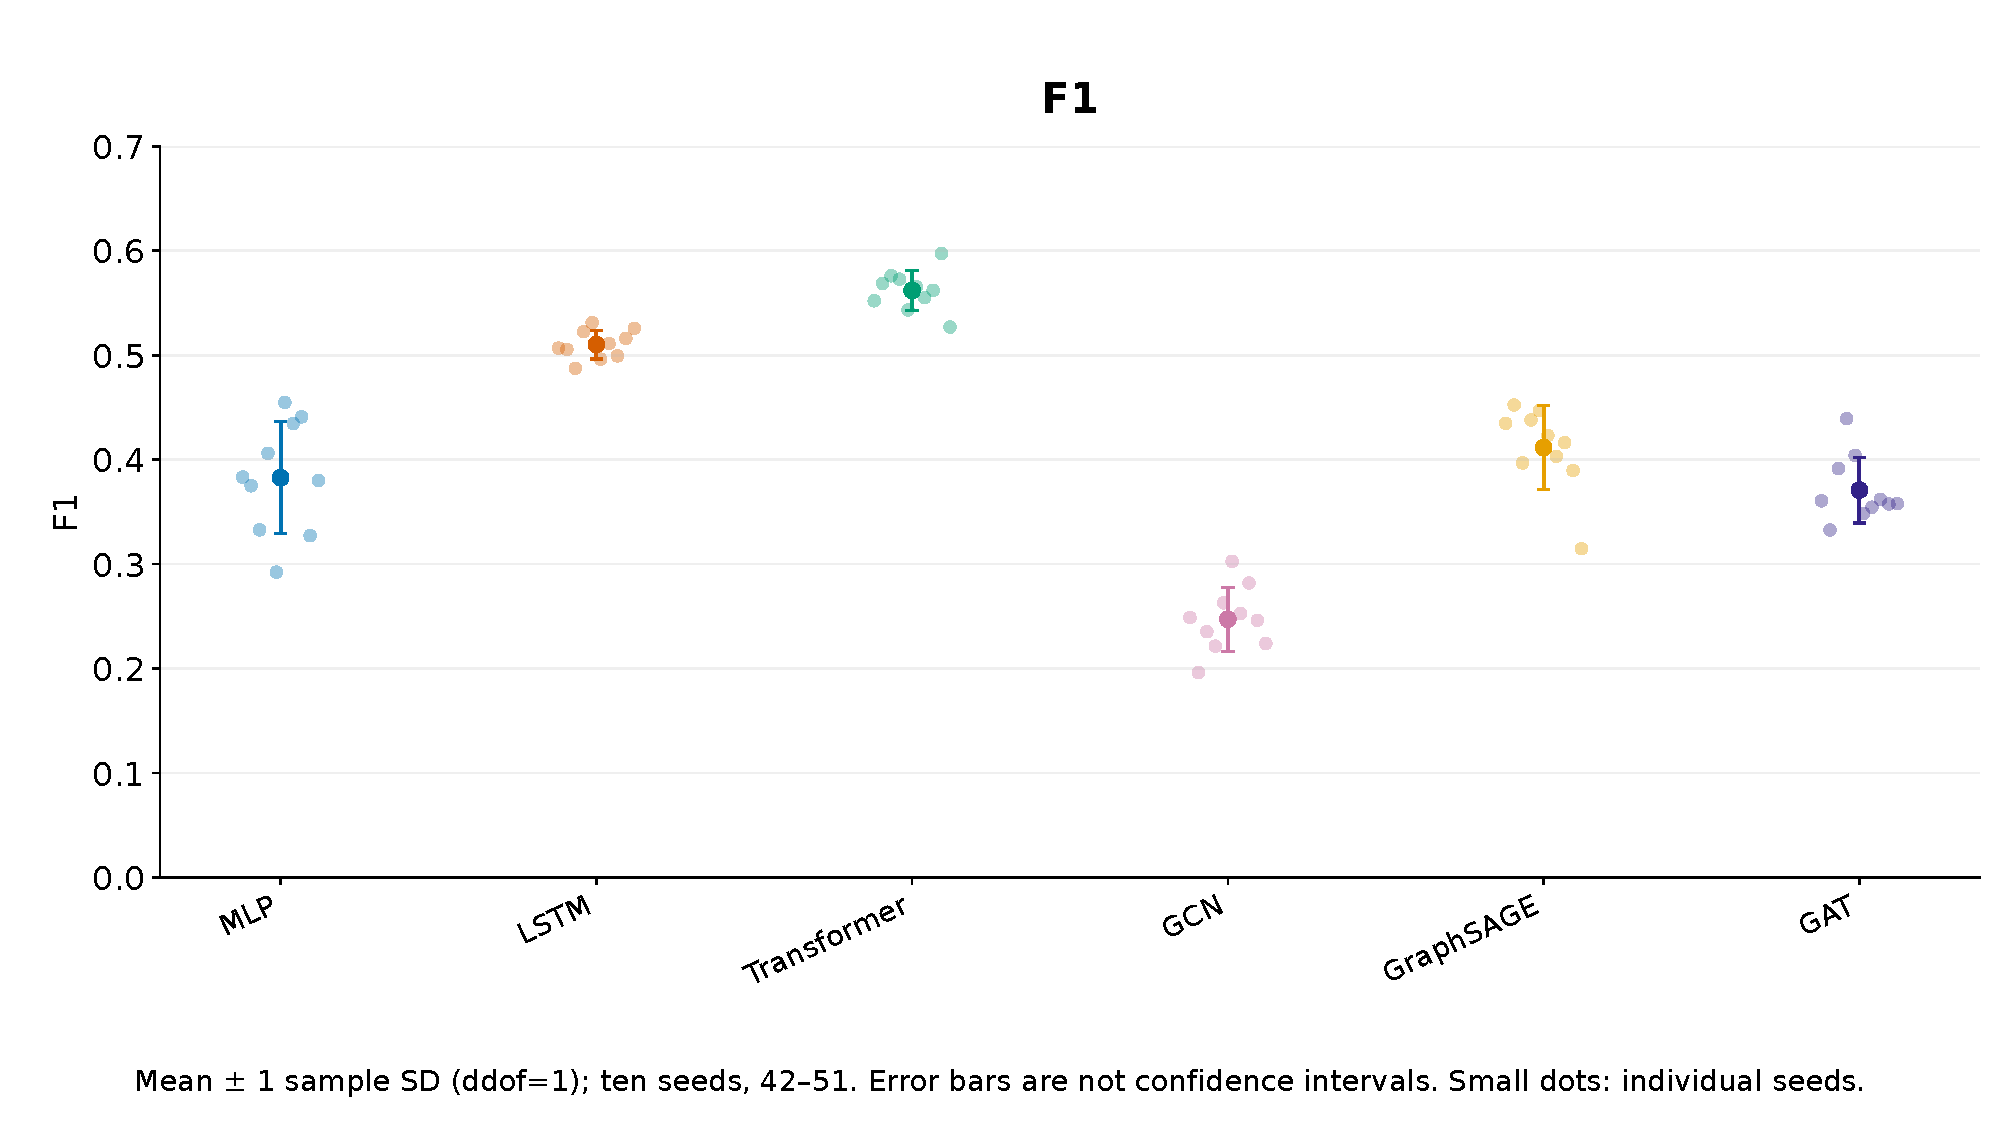
\includegraphics[width=\linewidth]{thesis_figures/slides/f1_score/03_results_elliptic.pdf}
\caption{Elliptic: ten-seed means $\pm$ sample SD; GNNs use the native graph. AP is average precision. F1 and recall use validation-selected thresholds. }
\label{fig:f1-score/03-results-elliptic}
\end{figure}

\begin{figure}[htbp]
\centering
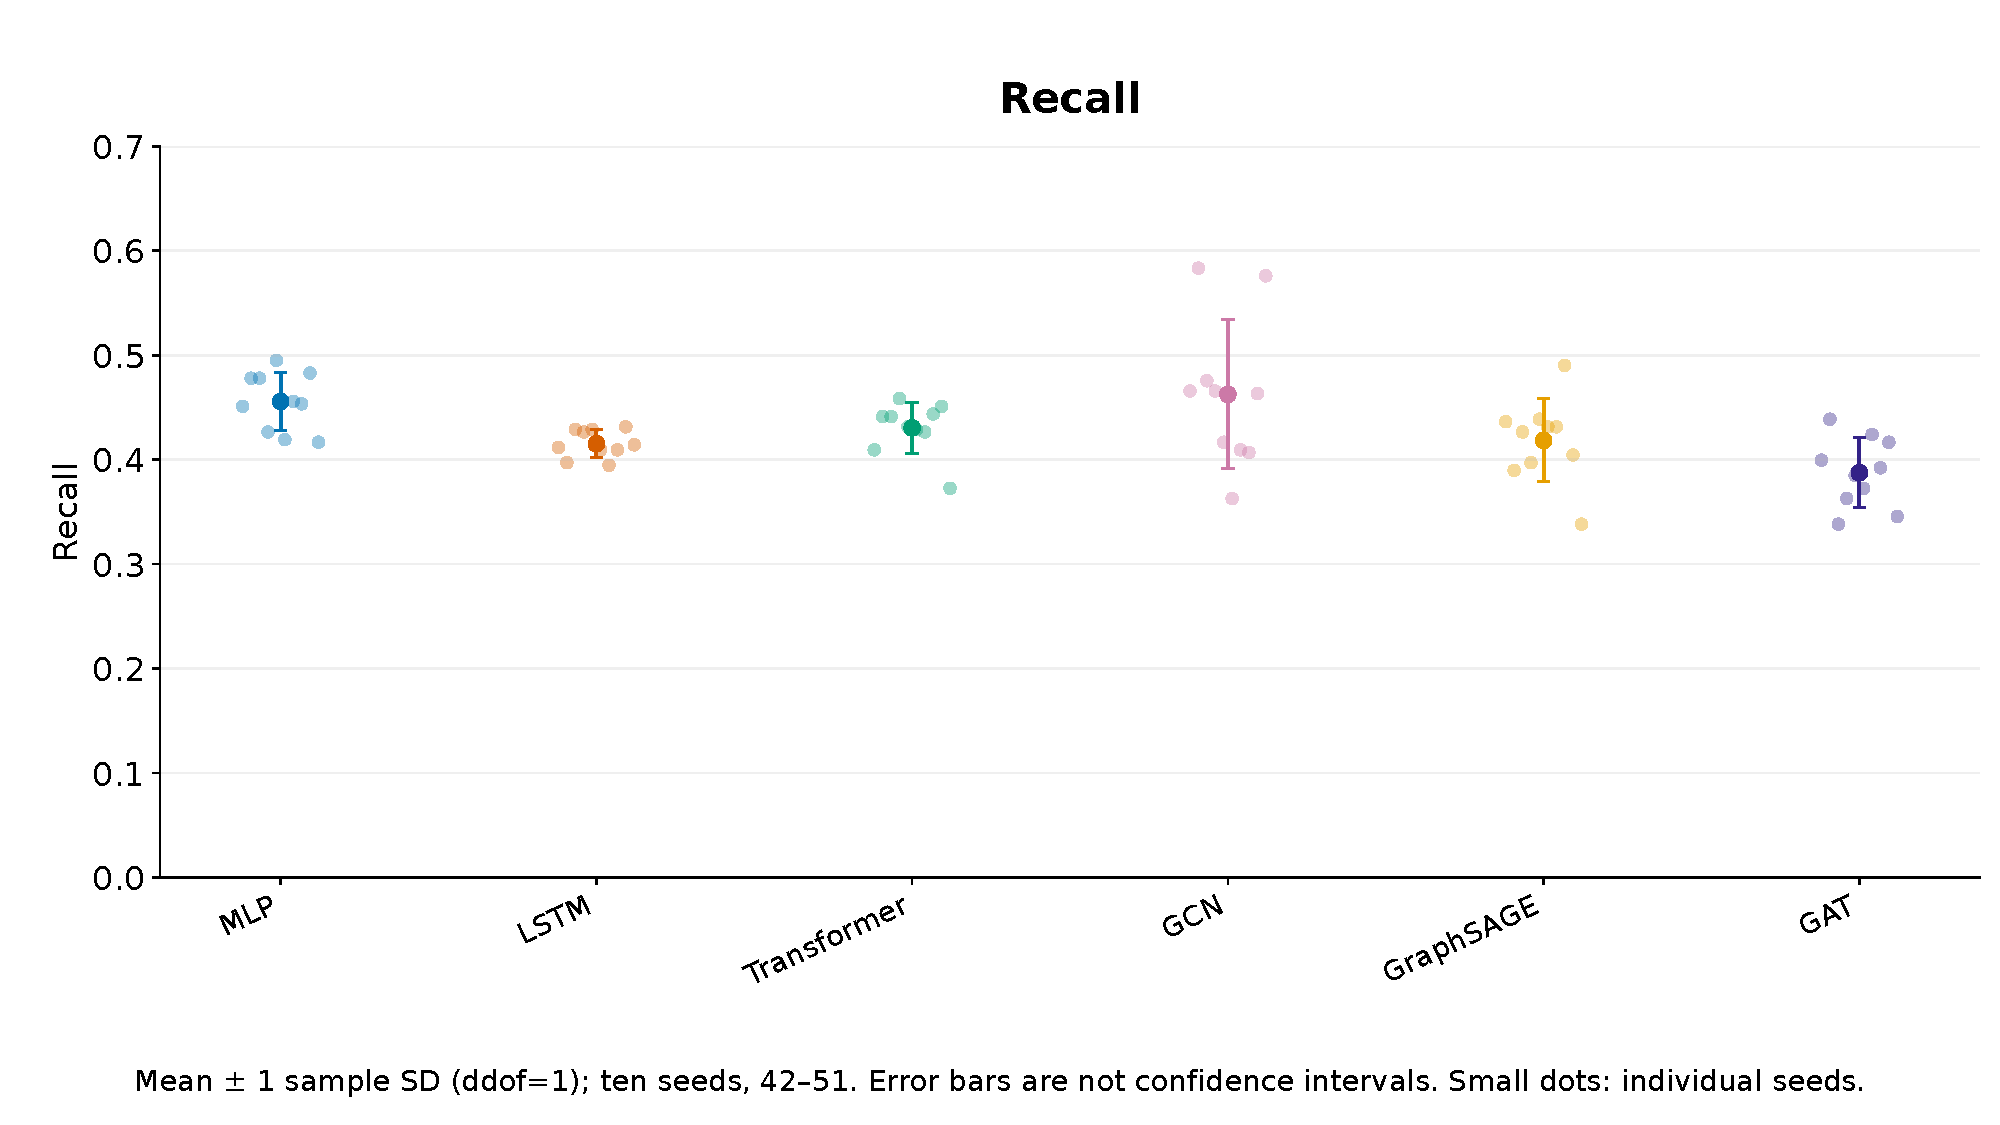
\includegraphics[width=\linewidth]{thesis_figures/slides/recall/03_results_elliptic.pdf}
\caption{Elliptic: ten-seed means $\pm$ sample SD; GNNs use the native graph. AP is average precision. F1 and recall use validation-selected thresholds. }
\label{fig:recall/03-results-elliptic}
\end{figure}

\begin{figure}[htbp]
\centering
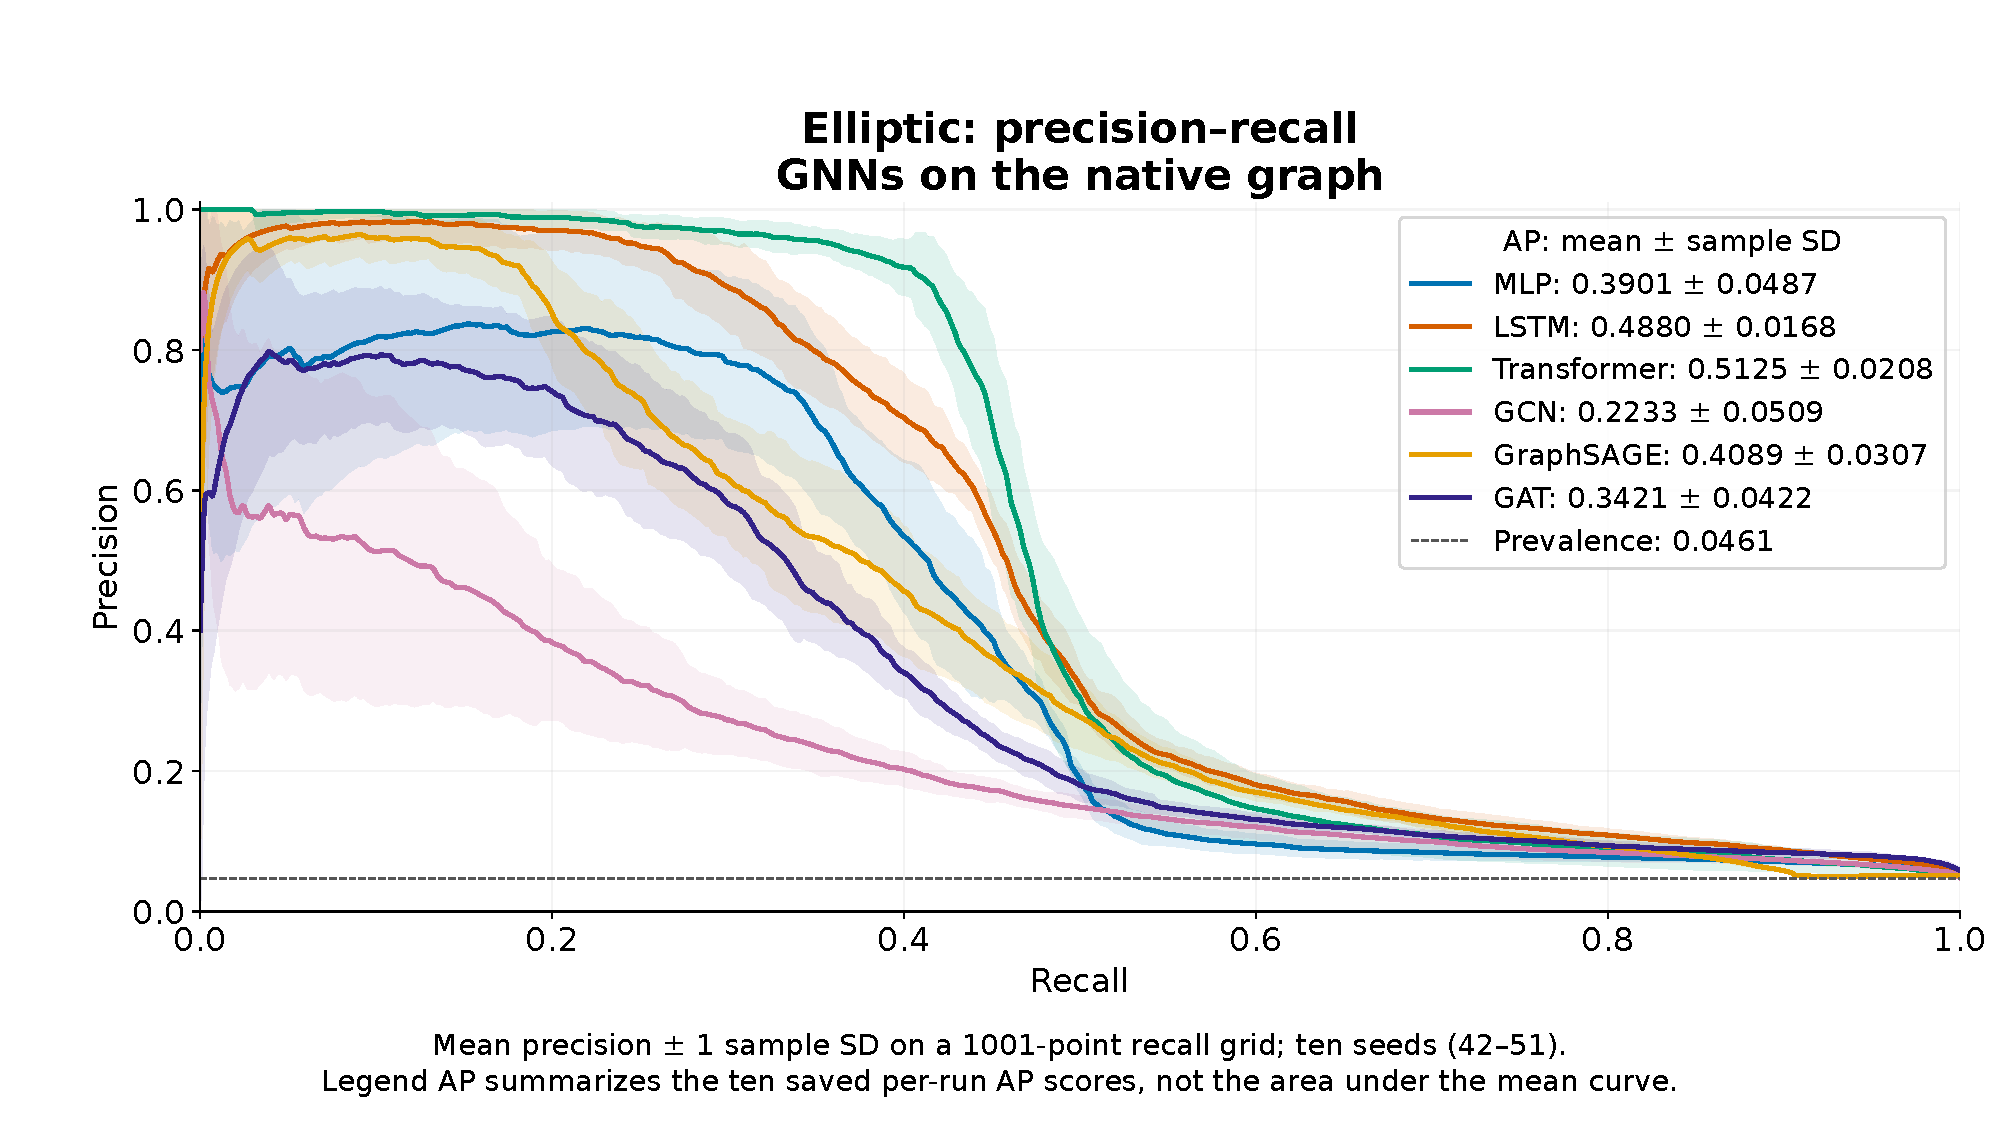
\includegraphics[width=\linewidth]{thesis_figures/slides/04_pr_curves_elliptic.pdf}
\caption{Elliptic; GNNs on the native graph. Mean precision curve and $\pm$1 sample-SD band across seeds 42--51, interpolated on 1001 common recall points. The synthetic (recall=0, precision=1) endpoint is removed first; at duplicate recall levels the first reversed point is retained, with constant endpoint extrapolation. Bands are clipped to [0,1]. Legend AP is the mean $\pm$ sample SD of the saved per-run AP scores, matching the ten-seed result tables; it is not the integrated mean curve. Each curve uses its validation-selected checkpoint; checkpoint paths and hashes appear in pr\_curve\_sources.csv.}
\label{fig:04-pr-curves-elliptic}
\end{figure}

\begin{figure}[htbp]
\centering
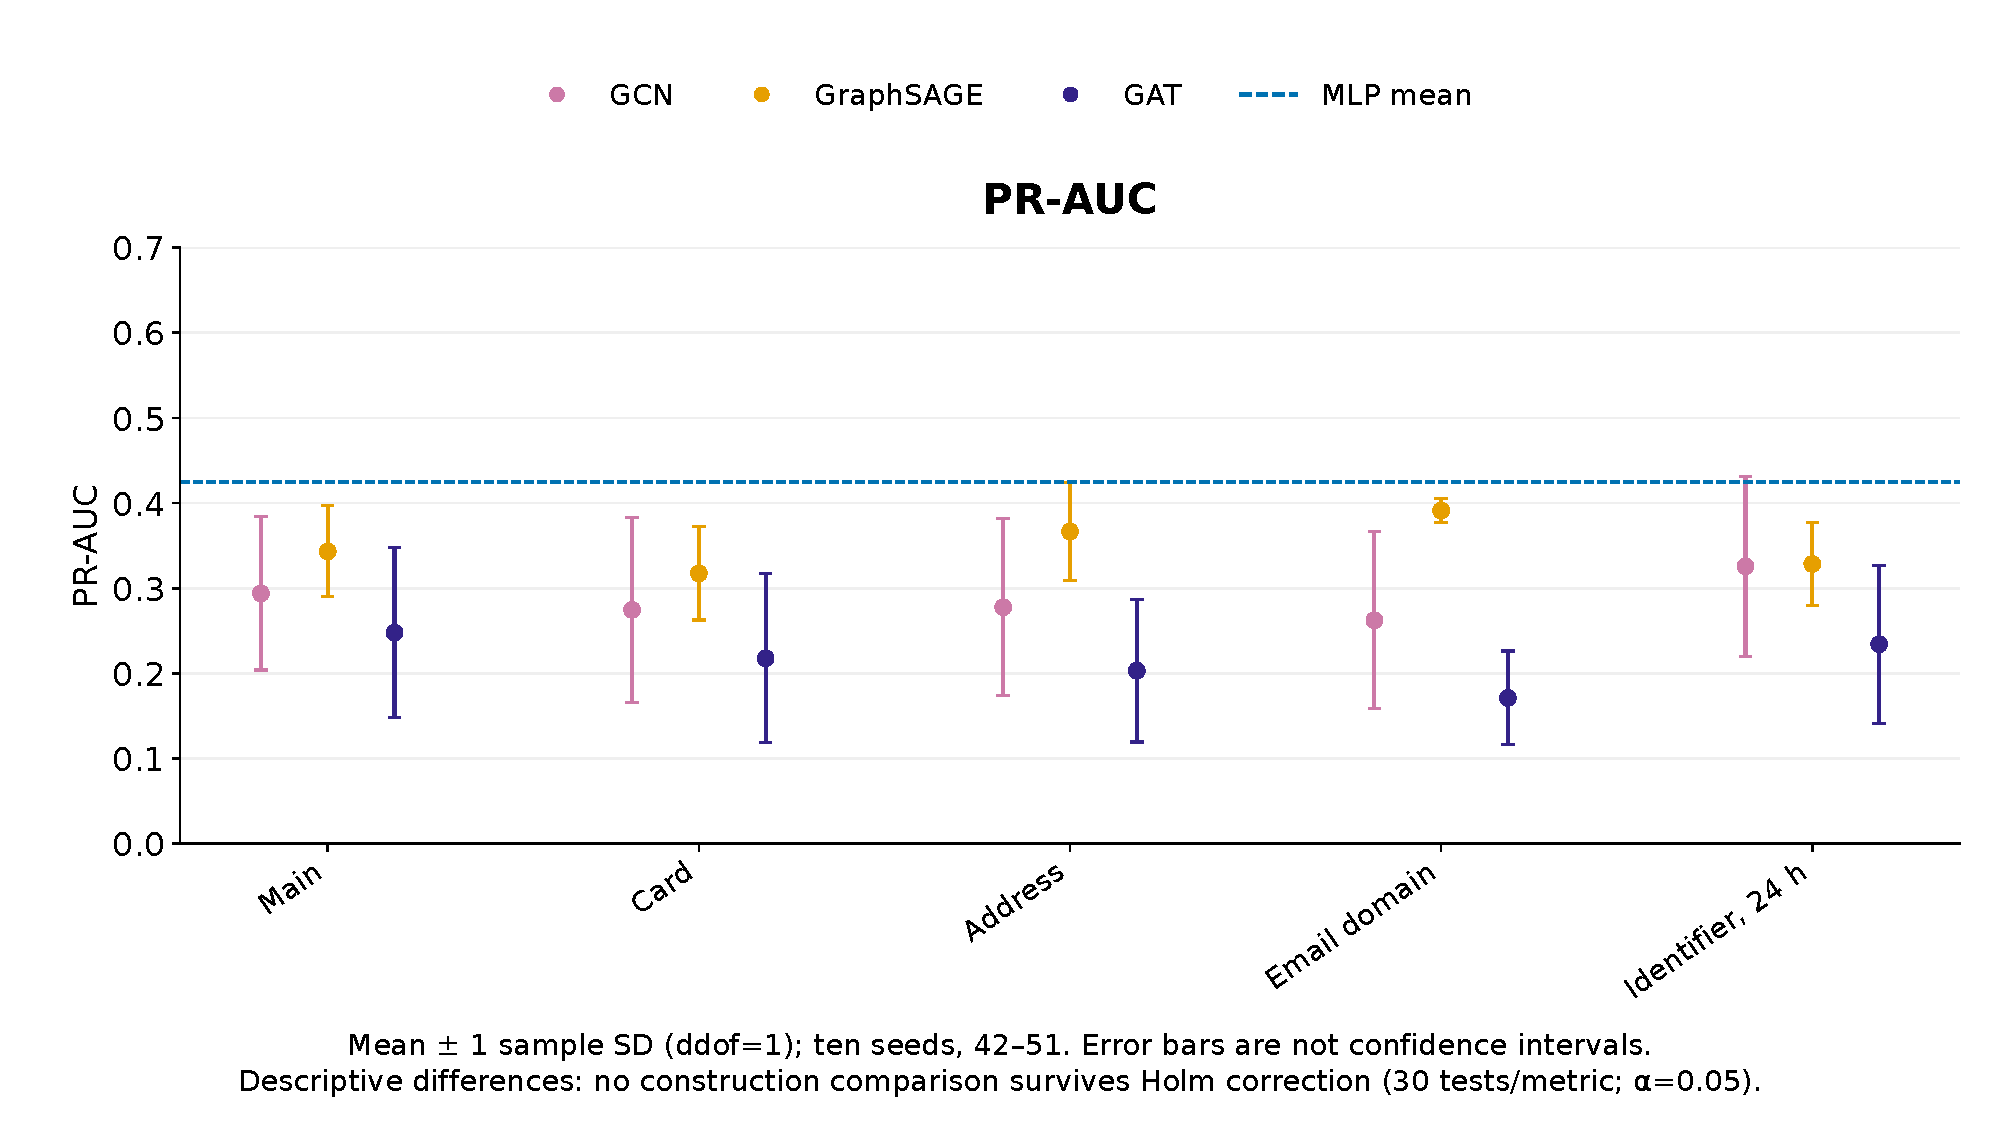
\includegraphics[width=\linewidth]{thesis_figures/slides/pr_auc/05_graph_construction_results.pdf}
\caption{IEEE-CIS construction comparison: ten-seed means $\pm$ sample SD. Dashed blue lines are the MLP means from the same saved result set. No construction comparison survives the prespecified Holm correction over 30 hypotheses per metric; descriptive improvements do not establish significance or equivalence.}
\label{fig:pr-auc/05-graph-construction-results}
\end{figure}

\begin{figure}[htbp]
\centering
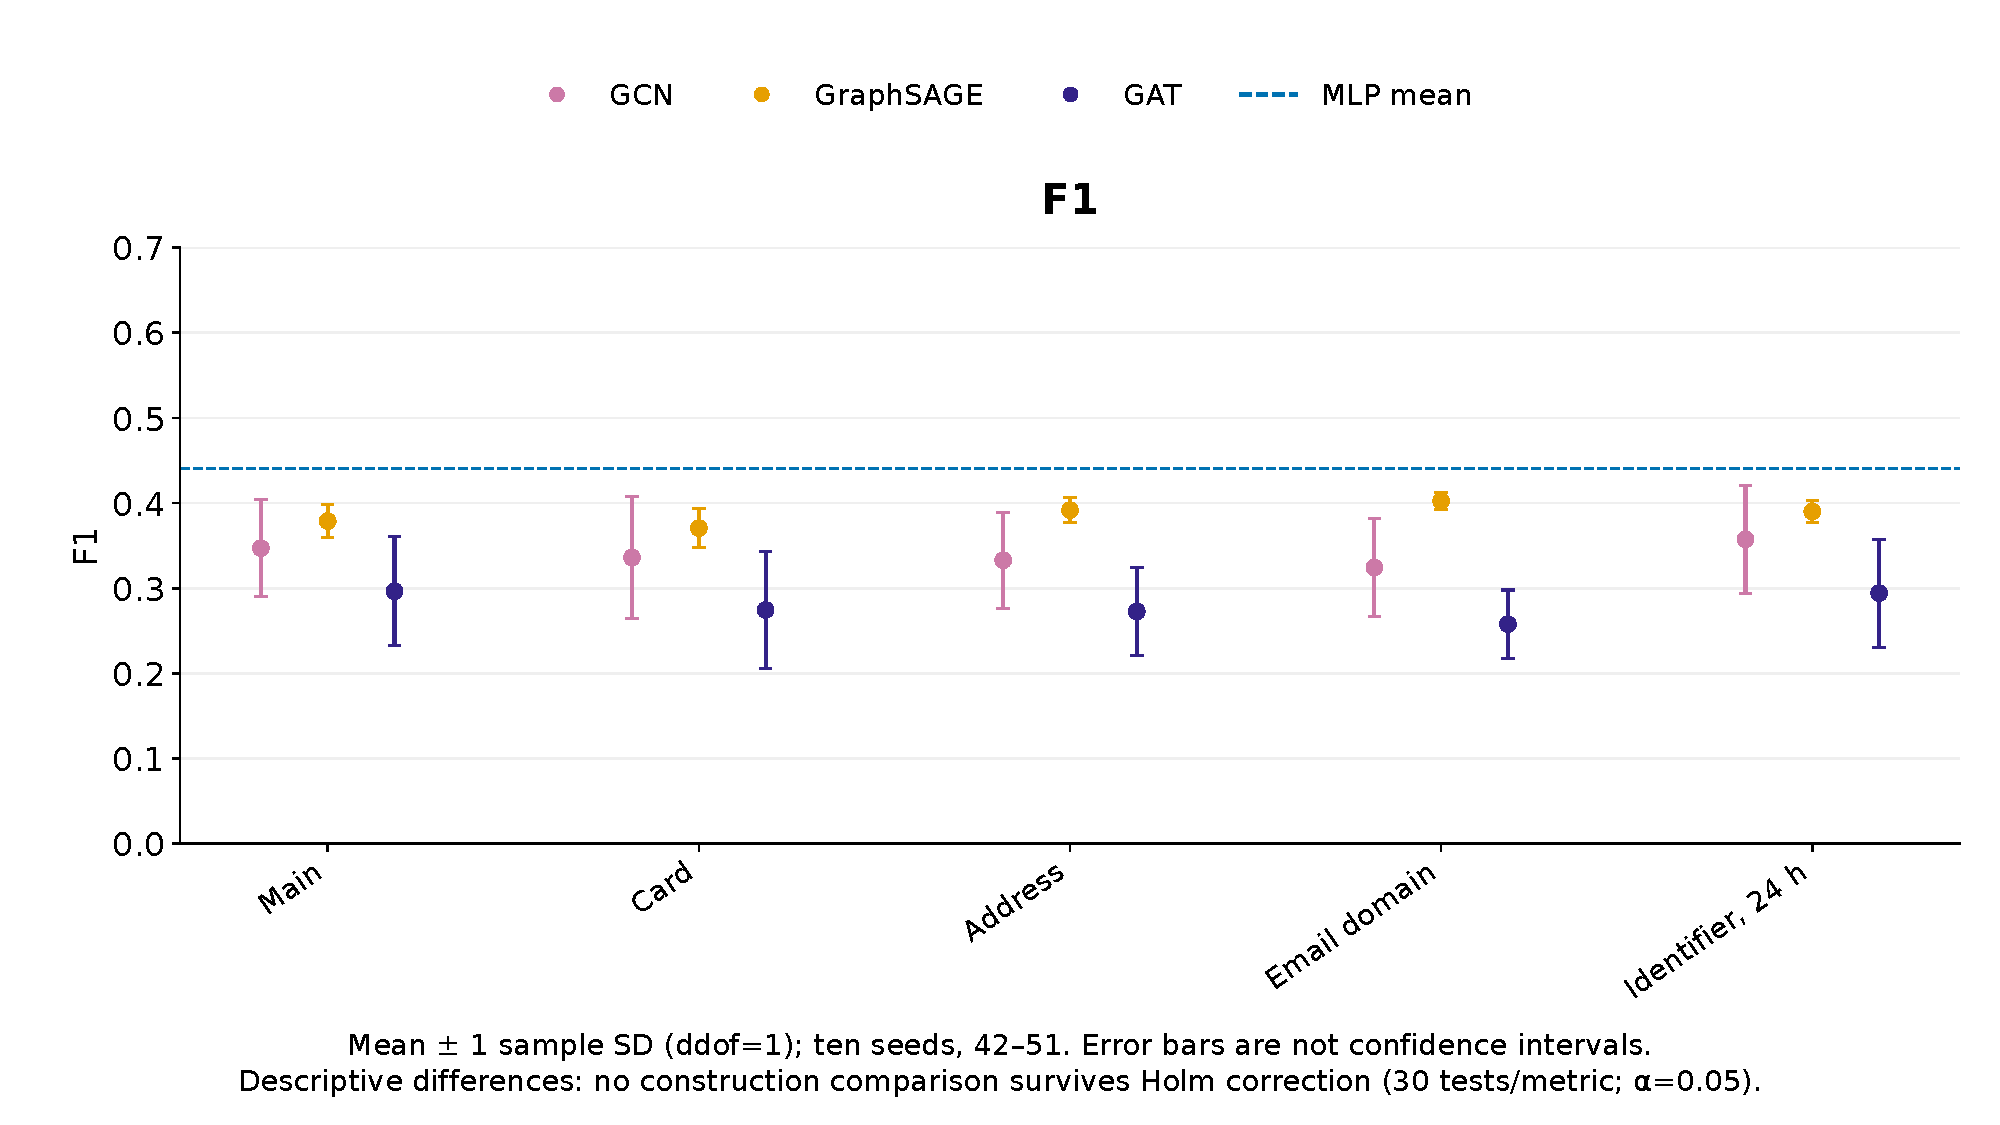
\includegraphics[width=\linewidth]{thesis_figures/slides/f1_score/05_graph_construction_results.pdf}
\caption{IEEE-CIS construction comparison: ten-seed means $\pm$ sample SD. Dashed blue lines are the MLP means from the same saved result set. No construction comparison survives the prespecified Holm correction over 30 hypotheses per metric; descriptive improvements do not establish significance or equivalence.}
\label{fig:f1-score/05-graph-construction-results}
\end{figure}
